\documentclass{scrreprt}

% usepackages
\usepackage{amsmath,amssymb}
\usepackage{subfiles}
\usepackage{nicefrac}
\usepackage[amsmath,framed,thmmarks]{ntheorem}  
\usepackage{hyperref}
\usepackage{framed}
\usepackage{graphicx}

% shortcuts

% math general
\newcommand{\partialup}{\partial}

% theorem environments
\theoremstyle{definition}
\theorembodyfont{\itshape}      % try commenting this line
\theoremprework{}       % code to process before the theorem 
\theorempostwork{}      % code to process after the theorem 
\theoremseparator{:}    % could be a : for example
\newtheorem{theorem}{Theorem}[chapter]
\newtheorem{problem}[theorem]{Problem}
\newtheorem{assumption}[theorem]{Assumption}
\newtheorem{remark}[theorem]{Remark}
\newtheorem{definition}[theorem]{Definition}
\newtheorem{lemma}[theorem]{Lemma}
\newtheorem{corollary}[theorem]{Corollary}

\newcommand{\qedhere}{\ifmmode\qed\else\hfill\proofSymbol\fi}
\theoremstyle{nonumberplain}
\theoremheaderfont{\itshape}
\theorembodyfont{\normalfont}
\theoremsymbol{\ensuremath{\square}}
\newtheorem{proof}{Proof}
\qedsymbol{\ensuremath{\square}}

% vectors, matrices
\newcommand{\scal}[1]{\mathit{#1}}
\renewcommand{\vec}[1]{{\textbf{#1}}}
\newcommand{\stvec}[1]{\widetilde{\vec{#1}}}
\newcommand{\gvec}[1]{{\boldsymbol #1}}
\newcommand{\mat}[1]{{\textbf #1}}
\newcommand{\matel}[3]{#1_{#2\,#3}}
\newcommand{\gmat}[1]{{\boldsymbol #1}}
\newcommand{\vecel}[2]{\mathit{#1}_{#2}}
\newcommand{\gmatel}[3]{#1_{#2\,#3}}
\newcommand{\transp}{^\textrm{T}}
\newcommand{\trace}{\text{tr}}
\newcommand{\nullvec}{\mathbf{0}}

% analysis
\newcommand{\suprem}[1]{\textup{sup}_{#1}}

% linear algebra
\newcommand{\laVec}[1]{\underline{\mathrm{#1}}}
\newcommand{\laVecel}[1]{\mathrm{#1}}
\newcommand{\laMat}[1]{\underline{\mathrm{#1}}}
\newcommand{\laMatel}[1]{\mathrm{#1}}
\newcommand{\laSpace}[1]{\mathbb{R}^{#1}}

% geometry
\newcommand{\point}{\vec{x}}
\newcommand{\domain}{\Omega}
\newcommand{\domainClosed}{\overline{\domain}}
\newcommand{\boundary}{{\partialup\domain}}
\newcommand{\boundaryD}{{\boundary_\textup{D}}}
\newcommand{\boundaryN}{{\boundary_\textup{N}}}
\newcommand{\boundaryM}{{\boundary_\textup{n}}}
\newcommand{\boundaryIn}{{\boundary_{-}}}
\newcommand{\boundaryOut}{{\boundary_{+}}}
\newcommand{\inDomain}{\textup{in }\domain}
\newcommand{\onBoundary}{\textup{on }\boundary}
\newcommand{\onBoundaryD}{\textup{on }\boundaryD}
\newcommand{\onBoundaryN}{\textup{on }\boundaryN}
\newcommand{\onBoundaryM}{\textup{on }\boundaryM}
\newcommand{\neumannVec}{\vec{g}_\textup{N}}
\newcommand{\neumannVecel}{g_{\textup{N},i}}
\newcommand{\dirichletVec}{\vec{g}_\textup{D}}
\newcommand{\dirichletVecel}{g_{\textup{D},i}}
\newcommand{\navierNeumann}{g_\textup{n,t}}
\newcommand{\navierDirichlet}{g_\textup{n,n}}
\newcommand{\inflow}{g_{-}}
\newcommand{\normal}{\vec{n}}
\newcommand{\normalT}[1]{\vecel{n}{#1}}
\newcommand{\tangential}{\vec{t}}
\newcommand{\tangentialT}[1]{\vecel{t}{#1}}

% mesh 
\newcommand{\triaClosed}{\bar{\mathcal{E}}_h}
\newcommand{\tria}{\mathcal{T}_h}
\newcommand{\cell}{K}
\newcommand{\Ncell}{{N_{\cell}}}
\newcommand{\cellClosed}{\bar{\cell}}
\newcommand{\cellNormal}[1]{\vec{n}^{{#1}}}
\newcommand{\cellNormalT}[2]{n_{#2}^{{#1}}}
\newcommand{\cellTangent}[1]{\vec{t}^{{#1}}}
\newcommand{\cellTangentT}[2]{t_{#2}^{{#1}}}
\newcommand{\cellPlus}{{\cell^+}}
\newcommand{\cellMinus}{{\cell^-}}
\newcommand{\cellBnd}{{\partialup\cell}}
\newcommand{\cellBndPlus}{{\partialup\cellPlus}}
\newcommand{\cellBndMinus}{{\partialup\cellMinus}}
\newcommand{\face}{e}
\newcommand{\nCellFaces}{{N_\face}}
\newcommand{\skeleton}{\Gamma}
\newcommand{\internalFaces}{\Gamma_h}
\newcommand{\skeletonD}{{\skeleton_\textup{D}}}
\newcommand{\skeletonN}{{\skeleton_\textup{N}}}
\newcommand{\skeletonM}{{\skeleton_\textup{n}}}
\newcommand{\sumDim}{\sum_{i=1}^d}
\newcommand{\sumDims}{\sum_{i,\idx{j}=1}^d}
\newcommand{\sumCellFaces}{\sum_{i=1}^{\nCellFaces}}
\newcommand{\sumCells}{\sum_{\cell \in \tria}}
\newcommand{\sumInternalFaces}{\sum_{\face\in\internalFaces}}
\newcommand{\sumSkeletonD}{\sum_{\face\in\skeletonD}}
\newcommand{\sumSkeletonM}{\sum_{\face\in\skeletonM}}
\newcommand{\sumSkeletonN}{\sum_{\face\in\skeletonN}}
\newcommand{\sumFaces}{\sum_{\face \in \internalFaces \cup \skeletonD}}
\newcommand{\sumFacesImpl}{\sum_{\face \in \internalFaces \cup \skeletonD \cup \skeletonM}}
\newcommand{\sumNeumann}{\sum_{\face \in \boundaryN}}
\newcommand{\hmax}{h_\textup{max}}
\newcommand{\hcell}{h_\cell}
\newcommand{\hcellPlus}{h_\cellPlus}
\newcommand{\hcellMinus}{h_\cellMinus}
\newcommand{\hface}{h_\face}
\newcommand{\kmax}{k_\textup{max}}
\newcommand{\kface}{k_\face}
\newcommand{\kcell}{k_\cell}
\newcommand{\kcellPlus}{k_\cellPlus}
\newcommand{\kcellMinus}{k_\cellMinus}
\newcommand{\lcell}{l_\cell}

\newcommand{\dt}{\textup{d}t}

% integrals
\newcommand{\dV}{\text{d}\vec{x}}
\newcommand{\ds}{\text{d}s}
\newcommand{\intDomain}{\int_\domain}
\newcommand{\intBoundary}{\int_\boundary}
\newcommand{\intCell}{\int_\cell}
\newcommand{\intFace}{\int_\face}

% mapping
\newcommand{\refVec}[1]{\hat{\vec{#1}}}
\newcommand{\refCell}{\hat{\cell}}
\newcommand{\refFace}{\hat{\face}}
\newcommand{\mapping}{\boldsymbol{\mathcal{F}}_{\cell}}
\newcommand{\mappingT}[1]{\mathcal{F}_{\cell,#1}}
\newcommand{\imapping}{\boldsymbol{\mathcal{F}}^{-1}_{\cell}}
\newcommand{\jacobian}{\textup{D}\boldsymbol{\mathcal{F}}_{\cell}}
\newcommand{\jacobianT}[2]{\frac{\partialup \mathcal{F}_{\cell,#1}}{\partialup
{#2}}}
\newcommand{\detJ}{J_\cell}
\newcommand{\ijacobian}{\textup{D}\vec{F}_{\cell}^{-1}}
\newcommand{\intRefCell}{\int_{\hat{\cell}}}
\newcommand{\refdV}{\textup{d}\hat{\vec{x}}}
\newcommand{\refdx}{\textup{d}\hat{x}}
\newcommand{\refdy}{\textup{d}\hat{y}}

\newcommand{\mappingst}{\boldsymbol{\mathcal{F}}_{\cell,t}}
\newcommand{\imappingst}{\boldsymbol{\mathcal{F}}^{-1}_{\cell,t}}

\newcommand{\reft}{\hat{t}}
\newcommand{\refdt}{\textup{d}\hat{t}}

% discrete function spaces
\newcommand{\spans}[1]{\textup{span}\left\{#1\right\}}
\newcommand{\polyspace}[3]{\mathit{#1}_{#2}(#3)}
\newcommand{\polyspaceVec}[3]{\vec{#1}_{#2}(#3)}

\begin{document}

\title{ADER-DG Implementation}
\author{Dominic Etienne Charrier}
\date{\today}
\maketitle

%%%%%%%%%%%%%%%%%%%%%%%%%%%%%%%%%%%%%%%%%%%%%%%%%%%%%%%%%%%%%%%
%%%%%%%%%%%%%%%%%%%%%%%%%%%%%%%%%%%%%%%%%%%%%%%%%%%%%%%%%%%%%%%
\chapter{ADERDG Implementation}
%%%%%%%%%%%%%%%%%%%%%%%%%%%%%%%%%%%%%%%%%%%%%%%%%%%%%%%%%%%%%%%
%%%%%%%%%%%%%%%%%%%%%%%%%%%%%%%%%%%%%%%%%%%%%%%%%%%%%%%%%%%%%%%
\section{Notation}
\begin{itemize}
  \item Scalar quantities with physical meaning (coordinates, pressures, \ldots)
  are written in italic letters.
  This also includes the components of vectors and tensors with physical meaning;
  see the next bullet point.
  \item Vectors and tensors with physical meaning (points, velocities, forces,
  stresses,\ldots) are printed in bold and using upright letters, e.g.,
  $\mat{A}$, $\vec{f}$.
  \item Linear algebra vectors and matrices are written in upright letters
  and are underlined, e.g., $\laMat{A}$, $\laVec{f}$. Elements belonging to
  linear algebra vectors and matrices
  are also written in an upright font but are not underlined, e.g.
  $\laMatel{A}_{ij}$, $\laVecel{f}_i$.
\end{itemize}
%%%%%%%%%%%%%%%%%%%%%%%%%%%%%%%%%%%%%%%%%%%%%%%%%%%%%%%%%%%
%%%%%%%%%%%%%%%%%%%%%%%%%%%%%%%%%%%%%%%%%%%%%%%%%%%%%%%%%%%
\section{Computational mesh and trace operators}
\label{sec:mesh}
%%%%%%%%%%%%%%%%%%%%%%%%%%%%%%%%%%%%%%%%%%%%%%%%%%%%%%%%%%%
%%%%%%%%%%%%%%%%%%%%%%%%%%%%%%%%%%%%%%%%%%%%%%%%%%%%%%%%%%%
Let $\tria$ be a partition of the domain
$\domain\subset\mathbb{R}^d$ consisting of quadrilateral/hexahedral elements.
We refer to the disjoint open sets $\cell \in \tria$ as mesh cells. We denote by
$\hcell$ the diameter of $\cell$.
We store the local quantities $\hcell$ in the vector
$\laVec{h} = \{ \hcell \}_{\cell \in \tria}$, and
set
$h_\textup{max} = \text{max}_{\cell \in \tria }\,\hcell$.
Finally, $\normal$ denotes the outward normal unit vector to the cell boundary
$\cellBnd$. We will denote the number of cells by $\Ncell$.

An interior face of $\tria$ is the $d-1$ dimensional intersection
$\cellBnd^{+} \cap \cellBnd^{-}$, where $\cellPlus$ and $\cellMinus$
are two adjacent elements of $\tria$. Similarly, a boundary face of $\tria$ is
the $d-1$ dimensional intersection $\cellBnd \cap \boundary$ which consists
of entire faces of $\cellBnd$.
We denote by $\internalFaces$ the union of all interior faces of $\tria$.

Here and in the following, we refer generically to a ``face" even in the
case $d=2$.
%%%%%%%%%%%%%%%%%%%%%%%%%%%%%%%%%%%%%%%%%%%%%%%%%%%%%%%%%%%
%%%%%%%%%%%%%%%%%%%%%%%%%%%%%%%%%%%%%%%%%%%%%%%%%%%%%%%%%%%
\section{Mappings}
%%%%%%%%%%%%%%%%%%%%%%%%%%%%%%%%%%%%%%%%%%%%%%%%%%%%%%%%%%%
%%%%%%%%%%%%%%%%%%%%%%%%%%%%%%%%%%%%%%%%%%%%%%%%%%%%%%%%%%%
In this section, we introduce mappings between the mesh cells
$\cell\in\tria$ and a reference cell. Mappings allow
us to treat integrals over mesh cells with non-uniform extent in an
uniform manner.
To ease the presentation, we only consider the two-dimensional case here.
\\[5pt]
Let us define the \textit{reference cell} ${\refCell=[0,1]^2}$
and let us denote by $\refVec{x}=(\hat{x},\hat{y})\transp$ a point belonging to $\refCell$.
Let $\cell\in\tria$ denote a nondegenerate quadrilateral cell with
center $\vec{P}_0$ and cell size $(\Delta x,\,\Delta y)^T$.

We can express $\cell$ according to
\begin{align}
\cell &= \mapping (\refCell),
\notag
\intertext{where we define the mapping $\mapping : \refCell \to \cell$ as}
\label{eq:aderdg_impl:mapping:mapping_2d}
\vec{x} = \mapping(\refVec{x})
&=
\begin{pmatrix}
\mappingT{x}(\refVec{x})\\
\mappingT{y}(\refVec{x})
\end{pmatrix}
=
\vec{P}_0 +
\begin{pmatrix}
\Delta x & 0 \\
0 & \Delta y
\end{pmatrix}
\begin{pmatrix}
\hat{x}-0.5 \\ \hat{y}-0.5
\end{pmatrix}
\end{align}
We will further denote the inverse mapping by
$\imapping\colon\,\cell \to \refCell$.

The considered quadrilateral cells have a constant Jacobian matrix, i.e.,
\begin{align}
\label{eq:ader_impl:mappings:constant_jacobian}
\jacobian (\refVec{x})&=
\begin{pmatrix}
\jacobianT{x}{\hat{x}} & \jacobianT{x}{\hat{y}} \\
\jacobianT{y}{\hat{x}} & \jacobianT{y}{\hat{y}}
\end{pmatrix}(\refVec{x})
=
\begin{pmatrix}
\Delta x & 0 \\
0 & \Delta y
\end{pmatrix},
\notag
\intertext{and thus also a constant Jacobian determinant:}
\detJ(\refVec{x}) &= \textup{det}\left(\jacobian\right)(\refVec{x})\notag\\
&= \Delta x\,\Delta y.
\end{align}

Let $\hat{f}$ be a sufficiently regular function on the reference cell
$\refCell$. Further let $f$ be sufficiently regular on $\cell$ and such that
\begin{align}
\label{eq:aderdg_impl:imapping_scalar_function}
f(\vec{x}) &= (\hat{f} \circ \imapping)(\vec{x}) = \hat{f}(\refVec{x}),
\qquad
\refVec{x}\in\refCell,\,\vec{x}=\mapping(\refVec{x})\in\cell.
\end{align}
Then, it holds that
\begin{align}
\label{eq:aderdg_impl:mapping:gradient_2d}
\nabla\,f(\vec{x})
&= \left(\jacobian^{-\textup{T}}\,\cdot\hat{\nabla}\,\hat{f}\right)(\refVec{x})
=
\begin{pmatrix}
\frac{1}{\Delta x} & 0 \\
0 & \frac{1}{\Delta y}
\end{pmatrix}\,
\hat{\nabla}\,\hat{f}(\refVec{x})
\intertext{where}
\hat{\nabla} &= \left(\frac{\partial}{\partial \hat{x}},\,\frac{\partial}{\partial \hat{y}}\right)\transp
\notag
\end{align}
denotes the gradient with respect to the reference coordinates. This follows
from \eqref{eq:aderdg_impl:imapping_scalar_function} and using the chain rule.
A similar identity can be derived for vector-valued functions.

We can also express integrals over the volume of cell $\cell$
with respect to the reference coordinates and the invertible mapping $\mapping$.
Let $\hat{f}$ and $f$ be defined as in \eqref{eq:aderdg_impl:imapping_scalar_function},
we have
\begin{align}
\intCell f(\vec{x})\,\dV
&\overset{\phantom{\eqref{eq:ader_impl:mappings:constant_jacobian}}}{=}
\intRefCell \hat{f}(\refVec{x})\,|\detJ(\refVec{x})|\,\refdV
= \int_{0}^1\int_{0}^1
\hat{f}(\hat{x},\hat{y})\,|\detJ(\hat{x},\hat{y})|\,\refdx\,\refdy \notag\\
&\overset{\eqref{eq:ader_impl:mappings:constant_jacobian}}{=}
\detJ\,
\int_{0}^1\int_{0}^1
\hat{f}(\hat{x},\hat{y})\,\,\refdx\,\refdy
\notag\\
&\overset{\phantom{\eqref{eq:ader_impl:mappings:constant_jacobian}}}{=}
\Delta x\,\Delta y\,
\int_{0}^1\int_{0}^1
\hat{f}(\hat{x},\hat{y})\,\,\refdx\,\refdy.
\notag
\end{align}
Let us indicate the faces of the reference cell
using a tuple $(\xi, f)$, $\xi\in\{0,1,\ldots,d-1\}$, $f\in\{0,1\}$,
where the first index corresponds to the fixed coordinate direction:
\begin{align}
\refFace^{1,0} &= \{ \refVec{x} \in \refCell : \hat{x} = 0\},\qquad
\refFace^{1,1} =  \{ \refVec{x} \in \refCell : \hat{y} = 0\},
\notag\\
\refFace^{2,0} &= \{ \refVec{x} \in \refCell : \hat{x} = 1\},\qquad
\refFace^{2,1} =  \{ \refVec{x} \in \refCell : \hat{y} = 1\},
\notag
\end{align}
Then, we can define the four faces belonging to the boundary of $\cell$
according to:
\begin{align}
\face^{1,0} &= \mapping(\refFace^{1,0}),\qquad
\face^{1,1} =  \mapping(\refFace^{1,1}),\qquad
\face^{2,0} =  \mapping(\refFace^{2,0}),\qquad
\face^{2,1} =  \mapping(\refFace^{2,1}).
\notag
\end{align}
Now we can express integrals over faces belonging to the boundary of $\cell$ with respect to
the reference coordinates and the mapping $\mapping$.
Let $\hat{f}$ and $f$ be defined as in \eqref{eq:aderdg_impl:imapping_scalar_function},
we have

\begin{align}
\int_{\face^{1,0}} f(\vec{x})\,\ds(\vec{x}) &=
\int_{0}^1\hat{f}(0,\hat{y})\,\left|\frac{\partial
\mapping(0,\hat{y})}{\partial\,\hat{y}}\right|\,\refdy
\notag\\
&\overset{\textup{\eqref{eq:aderdg_impl:mapping:mapping_2d}}}{=}
\Delta y
\int_{0}^1\hat{f}(0,\hat{y})\,\,\refdy,
\\
%%%%
\int_{\face^{1,1}} f(\vec{x})\,\ds(\vec{x}) &=
\int_{0}^1\hat{f}(1,\hat{y})\,\left|\frac{\partial
\mapping(1,\hat{y})}{\partial\,\hat{y}}\right|\,\refdy
\notag\\
&\overset{\phantom{\textup{\eqref{eq:aderdg_impl:mapping:mapping_2d}}}}{=}
\Delta y
\int_{0}^1\hat{f}(1,\hat{y})\,\,\refdy,
\\
%%%%
\int_{\face^{2,0}} f(\vec{x})\,\ds(\vec{x}) &=
\int_{0}^1\hat{f}(\hat{x},0)\,\left|\frac{\partial
\mapping(\hat{x},0)}{\partial\,\hat{x}}\right|\,\refdx
\notag\\
&\overset{\textup{\eqref{eq:aderdg_impl:mapping:mapping_2d}}}{=}
\Delta x
\int_{0}^1\hat{f}(\hat{x},0)\,\,\refdx,
\\
%%%
\int_{\face^{2,1}} f(\vec{x})\,\ds(\vec{x}) &=
\int_{0}^1\hat{f}(\hat{x},1)\,\left|\frac{\partial
\mapping(\hat{x},1)}{\partial\,\hat{x}}\right|\,\refdx
\notag
\\
&\overset{\phantom{\textup{\eqref{eq:aderdg_impl:mapping:mapping_2d}}}}{=}
\Delta x
\int_{0}^1\hat{f}(\hat{x},1)\,\,\refdx,
\end{align}

\subsection{Mappings in arbitrary dimensions}

All concepts considered in the previous section naturally extend to
higher dimensions.
Let us consider in this sections a reference cell $\refCell\in[0,1]^d$.

For the Jacobian determinant, we obtain in this case:
\begin{align}
\detJ\,
&=
\prod_{\xi=1}^{d}
\Delta x_\xi.
\end{align}

For a volume integral, we obtain:
\begin{align}
\label{eq:ader_impl:mappings:volume_integral}
\int_\cell f(\vec{x})\,\dV
&=
\detJ\,
\int_{\refCell} f(\refVec{x})\,\dV
\notag
\\
&=
\prod_{\xi=1}^{d}
\Delta x_\xi
\,
\int_{\refCell} \hat{f}(\refVec{x})\,\refdV
\end{align}

And for an integral over a face $e^{\xi,f}$, $\xi\in\{1,2,\ldots,d\}$,
$f\in\{0,1\}$, we obtain:
\begin{align}
\label{eq:ader_impl:mappings:face_integral}
\int_{\face^{\xi,f}} f(\vec{x})\,\ds (\vec{x})
&=
\prod_{\zeta=1,\zeta\neq\xi}^{d}
\Delta x_\zeta
\,
\int_{\refFace^{\xi,f}} \hat{f}(\refVec{x})\,
\refds (\refVec{x})
\notag\\
&=
\frac{\detJ}{\Delta x_\xi}
\,
\int_{\refFace^{\xi,f}} \hat{f}(\refVec{x})\,
\refds (\refVec{x})
\end{align}

Let $\hat{f}$ be a sufficiently regular function on the reference cell $\refCell$, and
let $f$ be sufficiently regular on $\cell$ and such that
\begin{align}
\label{eq:aderdg_impl:imapping_scalar_function}
f(\vec{x}) &= (\hat{f} \circ \imapping)(\vec{x}) = \hat{f}(\refVec{x}),
\qquad
\refVec{x}\in\refCell,\,\vec{x}=\mapping(\refVec{x})\in\cell.
\notag
\end{align}
Then, partial derivatives of $f$ can be expressed with respect
to the reference coordinates according to:
\begin{align}
\label{eq:aderdg_impl:mapping:gradient}
\frac{\partial f(\vec{x})}{\partial x_\xi}
&=
\frac{1}{\Delta x_\xi}
\frac{\partial \hat{f}(\refVec{x})}{\partial
\hat{x}_\xi},
\end{align}
where $\xi\in\{1,2,\ldots,d\}$.

\subsection{Space-time mappings}
We can express the tuple $(\cell,[t^\cell,t^\cell+\Delta t])$ according to
\begin{align}
(\cell,[t^\cell,t^\cell+\Delta t]) &= \mappingst (\refCell,[0,1]),
\notag
\intertext{where we have introduced the space-time mapping $\mappingst\colon\,
\refCell\times[0,1] \to \cell\times[t^K,t^K+\Delta t]$ with:}
\label{eq:aderdg_impl:mapping}
(\vec{x},t) = \mappingst(\refVec{x})
&=
(\vec{P}_0, t^K) +
\begin{pmatrix}
\Delta x &        0 &        0 \\
0        & \Delta y &        0  \\
0        &        0 & \Delta t
\end{pmatrix}
\begin{pmatrix}
\hat{x}-0.5 \\ \hat{y}-0.5 \\ \hat{t}
\end{pmatrix}.
\end{align}

\section{Basis functions}
Let be $f$ be a sufficiently regular univariate function such that it
can be approximated by a polynomial of order $N$, i.e.,
the leading approximation error term is of order $\mathcal{O}(N+1)$.

Given a set of support point and function value pairs $\{(x_i,f(x_i))\}_{0\leq
i\leq N}$, the corresponding prolongation polynomial in the Lagrange form
can be constructed according to:
\begin{align}
f_N (x) &= \sum_{i=0}^{N}\,f(x_i)\,\varphi_i(x),
\intertext{where the Lagrange basis polynomials are defined as}
L_i(x) &=
\left(\prod_{\begin{smallmatrix}0\le l\le N\\ l\neq i\end{smallmatrix}}
\frac{x-x_l}{x_i-x_l}\right),
\qquad i = 0,\ldots,N,
\notag
\intertext{Since we exclude the $(x-x_i)$ term in the product, the basis
functions have the property} L_i(x_j) &=
\label{eq:aderdg_impl:lagrange_basis:discrete_nodal_orthogonality}
\delta_{ij}
=
\begin{cases}
1 &i=j,\\
0 &\textup{else}.
\end{cases}
\qquad i,j = 0,\ldots,N,
\end{align}

Let $I\in\mathbb{R}$ be a real interval.
With respect to the Gauss-Legendre quadrature of degree $2\,(N+1)-1$,
we define a discrete scalar product
$\langle \cdot,\cdot \rangle_{L^2(I)}$ according to:
\begin{align*}
\langle f,g\rangle_{L^2(I)} =
\sum_{n=0}^N\,w_n\,f(x_n)\,g(x_n),
\end{align*}
where $x_n$ denotes a quadrature node and $w_n$ denotes a quadrature
weight, $n=0,1,\ldots,N$.

The next result is very important for the definition of the DG basis
functions:
\begin{lemma}
Let us denote by $\{\varphi_{i}\}_{i=0,1,\ldots,N}$ a Lagrange basis utilising
basis polynomials located at the nodes of a Gauss-Legendre quadrature of
degree $2\,(N+1)-1$. Let the nodes lie in the interval $I$.
Then, $\{\varphi_{i}\}_{i=0,1,\ldots,N}$ is a orthogonal
basis with respect to the $(\cdot,\cdot)_{L^2(I)}$ scalar product.
Furthermore, it is a orthogonal basis with respect to all
Gauss-Legendre quadratures with at least a degree
of $2\,(N+1)-1$ that are used to evaluate $(\cdot,\cdot)_{L^2(I)}$.
\end{lemma}
\begin{proof}
We only need to proof that the basis functions are orthogonal with
respect to the Gauss-Legendre quadrature of degree $2\,(N+1)-1$.
The rest follows from the fact that the Gauss-Legendre
quadrature of degree ${2\,(N+1)-1}$ is exact for all polynomials of degree
$2\,(N+1)-1 > 2\,N$, where $2\,N$ is the maximum total degree
of the product of two basis polynomials.

Select two basis functions $\varphi_{i}$ and
$\varphi_{j}$,$i,j=0,1,\ldots,N$.
Since both functions are Lagrange polynomials, we have
\begin{align}
\label{eq:preliminaries:lagrange_orthogonality}
\varphi_i (x_j) =
\delta_{ij} =
\begin{cases}
1 & i=j, \\
0 & \textup{else},
\end{cases}
\end{align}
where $x_j$ denotes a support point, and $\delta_{ij}$ denotes the
Kronecker delta.
An analogous condition holds for $\varphi_j$.

We want to evaluate the scalar product
$(\cdot,\cdot)_{L^2(I)}$ by using the Gauss-Legendre
quadrature of degree $2\,(N+1)-1$.
We obtain:
\begin{align*}
(\varphi_i,\,\varphi_j)_{L^2(I)}
&=
\langle\varphi_i,\,\varphi_j\rangle_{L^2(I)}
=
\sum_{n=0}^{N} w_n\,\varphi_{i}(x_n)\,\varphi_{j}(x_n) =
\sum_{n=0}^{N} w_n\,\delta_{ij}\,\delta_{nj} =
w_i\,\delta_{ij}.
\end{align*}
\end{proof}
\subsection{Definition of the DG basis functions}
Let us introduce the space of polynomials of order
at most $N$ with support in $[0,\,1]$:
\begin{align*}
\polyspace{Q}{N}{[0,\,1]} &= \text{span}\left\{
\hat{x}^{n}\; \text{ such that }
0\leq n \leq N \textup{ and }\hat{x} \in [0,\,1] \right\}.
%\polyspace{Q}{N}{\refCell} &= \text{span}\left\{ \Pi_{i=1}^d\,
%x_i^{n_i}\; \text{ such that }n_i \in \mathbb{N}_0 \text{ and }
%n_i \leq N,\,i=1,\ldots,d,\, \text{ and } \vec{x} \in \cell \right\}.
\end{align*}
As a basis of the space
$\polyspace{Q}{N}{[0,1]}$,
we use a set of $N+1$ Lagrange basis polynomials.
The support points of the basis polynomials are chosen such that
they coincide with the nodes of a Gauss-Legendre quadrature of degree
$2\,(N+1)-1$ which uses the interval $[0,\,1]$
as domain of integration. We denote the scalar-valued univariate reference basis
functions by $\hat{\varphi}_i(\hat{x})$, $i=0,1,\ldots,N$.

Let us define scalar-valued multivariate polynomials on the reference cell
$\refCell=[0,1]^d$,
and on each mesh cell $\cell\in\tria$
according to:
\begin{align}
\label{eq:ader_impl:basis:basis_definition_ref_3d}
\hat{\phi}_n (\refVec{x}) &=
\prod^{d}_{\xi=1}
\hat{\varphi}_{n_\xi} (\hat{x}_\xi),
\\
\label{eq:ader_impl:basis:basis_definition_mesh_3d}
\phi^{K}_n (\vec{x}) &=
\begin{cases}
(\hat{\phi}_n \circ \imapping) (\vec{x}) & \vec{x}\in\cell,
\\
0 & \textup{else},
\end{cases}
\end{align}
for $n_\xi=0,1,\ldots,N$, $n_\xi\in\{1,\ldots,d\}$,
and a linearised index $n=0,1,\ldots,(N+1)^{d}-1$
that is constructed according to:
\begin{align*}
n = \sum_{\xi=1}^{d} N_\xi\,n_\xi,
\end{align*}
using the one-dimensional basis indices $n_\xi={0,1,\ldots,N}$ and some strides
$N_\xi\in\{0,N+1\}$, $\xi \in \{1,2,\ldots,d\}$ that define an unique order of
the degrees of freedom.

Notice that \eqref{eq:ader_impl:basis:basis_definition_mesh_3d} implies that
\begin{align*}
\vec{x} = \mapping \refVec{x}
\qquad
\Leftrightarrow
\qquad
\phi^{K}_n (\vec{x}) =
\hat{\phi}_n (\refVec{x}),
\end{align*}
for $\vec{x}\in\cell$, $\refVec{x}\in\refCell$,
and $n=0,1,\ldots,(N+1)^{d}-1$.

The corresponding $d$-dimensional support points ($d$-dimensional
Gauss-Legendre quadrature nodes) on the reference cell are constructed as tensor
products of the one-dimensional support points:
\begin{align*}
\refVec{x}_n = (\hat{x}_{n,1},\ldots,\hat{x}_{n,d})\transp,
\end{align*}
with $n=0,1,\ldots,(N+1)^{d}-1$.

One can show that the polynomials $\{\hat{\phi}_n
(\refVec{x})\}_{n=0,1,\ldots,(N+1)^d-1}$ form a basis of the space
\begin{align*}
\polyspace{Q}{N}{\refCell} &= \text{span}\left\{ \Pi_{i=1}^d\,
\hat{x}_i^{n_i}\; \text{ such that }
0 \leq n_i \leq N,\,i=1,\ldots,d,\, \text{ and } \refVec{x} \in \refCell
\right\}
\end{align*}
The $d$-dimensional support points for the multivariate
basis functions on the mesh cells
$\cell\in\tria$ are then constructed by means of the mapping $\mapping:$
\begin{align*}
(x_{n,1},\ldots,x_{n,d})\transp
&=
\mapping\refVec{x}_n,
\end{align*}
with $n=0,1\ldots,(N+1)^d-1$ denoting the global index.

Since we only consider affine reference cell to mesh cell mappings, we can
further show that the polynomials $\{{\phi}^K_n
(\vec{x})\}_{n=0,1,\ldots,(N+1)^d-1}$ form a basis of the space
\begin{align*}
\polyspace{Q}{N}{\cell} &= \text{span}\left\{ \Pi_{i=1}^d\,
x_i^{n_i}\; \text{ such that }
0 \leq n_i \leq N,\,i=1,\ldots,d,\, \text{ and } \vec{x} \in \cell
\right\}.
\end{align*}
Let us introduce another index $v=0,1,\ldots,N_\textup{var}-1$
that numbers the variables.
We construct the basis $\{{\phi}^{K;v}_n
(\vec{x})\}_{v=0,1,\ldots,N_\textup{var}-1;\;n=0,1,\ldots,(N+1)^d-1}$
of the space
$\polyspace{Q}{N}{\cell}^{N_\textup{var}}$ according to:
\begin{align*}
\{{\phi}^{K;v}_n
(\vec{x})\}&_{v=0,1,\ldots,N_\textup{var}-1;\;n=0,1,\ldots,(N+1)^d-1}
= \\
&\lbrace
(
1,\,
0,\,
\ldots,
0
)_{N_\textup{var}}\transp
,
(
0,\,
1,\,
\ldots,
0
)_{N_\textup{var}}\transp
,
\ldots,
,
(
0,\,
0,\,
\ldots,
1
)_{N_\textup{var}}\transp
\rbrace
\,\otimes
\\
&\{{\phi}^K_n
(\vec{x})\}_{n=0,1,\ldots,(N+1)^d-1}
\end{align*}

We further construct a basis $\{{\phi}^{K;v;e}_n
(\vec{x})\}_{e=1,2,\ldots,d;\;v=0,1,\ldots,N_\textup{var}-1;\;n=0,1,\ldots,(N+1)^d-1}$
of the space
$\polyspace{Q}{N}{\cell}^{N_\textup{var}\times d}$ according to:
\begin{align*}
\{{\phi}^{K;v;e}_n
(\vec{x})\}&_{e=1,2,\ldots,d;\;v=0,1,\ldots,N_\textup{var}-1;\;n=0,1,\ldots,(N+1)^d-1}
=
\\
&\lbrace
(
1,\,
0,\,
\ldots,
0
)_{N_\textup{var}}\transp
,
(
0,\,
1,\,
\ldots,
0
)_{N_\textup{var}}\transp
,
\ldots,
,
(
0,\,
0,\,
\ldots,
1
)_{N_\textup{var}}\transp
\rbrace
\,\otimes
\\
&\lbrace
(
1,\,
0,\,
\ldots,
0
)_{d}\transp
,
(
0,\,
1,\,
\ldots,
0
)_{d}\transp
,
\ldots
,
(
0,\,
0,\,
\ldots,
1
)_{d}\transp
\rbrace
\,\otimes
\\
&\{{\phi}^{K}_n(\vec{x})\}_{n=0,1,\ldots,(N+1)^d-1}
\end{align*}

Lastly, let us introduce the space-time basis polynomials
\begin{align*}
\hat{\theta}_{l;n} (\refVec{x},\hat{t}) &=
\hat{\varphi}_{l} (\hat{t})
\,
\hat{\phi}_{l;n} (\refVec{x},\hat{t})
\\
\theta^{K}_{l;n} (\vec{x},t) &=
\begin{cases}
(\hat{\theta}_{l;n} \circ \imappingst) (\vec{x},t) &
(\vec{x},t)\in\cell \times [t^K,t^K+\Delta t]  \\
0 & \textup{else},
\end{cases}
\end{align*}
with $l=0,1,\ldots,N$, and $n=0,1,\ldots,(N+1)^d-1$.
Here, $t^K$ denotes a time stamp associated with
the cell $\cell$.

The corresponding $(d+1)$-dimensional support points ($(d+1)$-dimensional
Gauss-Legendre quadrature nodes) on the reference cell are constructed as tensor
products of the one-dimensional support points:
\begin{align*}
(\refVec{x}_{n},\hat{t}_l) =
(\hat{x}_{n,1},\ldots,\hat{x}_{n,d},\hat{t}_l)\transp,
\end{align*}
with $n\in\{0,1,\ldots,(N+1)^{d}-1\}$ denoting the index of the spatial basis
and with $l\in\{0,1,\ldots,N\}$ denoting the index of the temporal basis.

We can now construct a basis $\{{\theta}^{K;v}_{l;n}
(\vec{x})\}_{v=0,1,\ldots,N_\textup{var}-1;\;l=0,1,\ldots,N;\;n=0,1,\ldots,(N+1)^d-1}$
of the space
$\polyspace{Q}{N}{\cell\times[t^K,t^K+\Delta t]}^{N_\textup{var}}$ according to:
\begin{align*}
\{{\theta}^{K;v}_{l;n}
(\vec{x})\}&_{v=0,1,\ldots,N_\textup{var}-1;\;l=0,1,\ldots,N;\;n=0,1,\ldots,(N+1)^d-1}
= \\
&\lbrace
(
1,\,
0,\,
\ldots,
0
)_{N_\textup{var}}\transp
,
(
0,\,
1,\,
\ldots,
0
)_{N_\textup{var}}\transp
,
\ldots,
,
(
0,\,
0,\,
\ldots,
1
)_{N_\textup{var}}\transp
\rbrace
\\
&\otimes
\{{\theta}^K_{l;n}
(\vec{x})\}_{l=0,1,\ldots,N;\;n=0,1,\ldots,(N+1)^d-1}.
\end{align*}
%%%%%%%%%%%%%%%%%%%%%%%%%%%%%%%%%%%%%%%%%%%%%%%%%%%%%%%%%%%
\subsection{Properties of the basis functions}
%%%%%%%%%%%%%%%%%%%%%%%%%%%%%%%%%%%%%%%%%%%%%%%%%%%%%%%%%%%
Let us number the $d$-dimensional Gauss-Legendre quadrature weights on the
reference cell with the linearised index
$n=0,1,\ldots,(N+1)^{d}-1$ we used to number the basis functions
and the corresponding $d$-dimensional spatial support points, i.e.,
\begin{align}
w_n = \prod_{\xi=1}w_{n_\xi},
\end{align}
with $n_\xi=0,1,\ldots,N$, $n_\xi\in\{1,\ldots,d\}$.

In this section, we summarise the properties of most of the
basis polynomials that appeared in the previous section.
We exclude the basis polynomials of the volume flux
and space-time volume flux ansatz spaces in the summary.
In the following, let $l,l'\in\{0,1,\ldots,N\}$,
$n,n'\in\{0,1,\ldots,(N+1)^d-1\}$,
$\cell,\cell'\in\tria$ and $v,v'\in\{0,1,\ldots,N_\textup{var}\}$.
The basis functions have the following properties:
\begin{itemize}
  \item Lagrange basis property (reference cell):
  \begin{align}
\label{eq:ader_impl:basis:lagrange_ref_1d}
{\hat{\varphi}}_{l} (\hat{x}_{l'}) &= \delta_{ll'},\\
{\hat{\phi}}_{n} (\refVec{x}_{n'}) &= \prod_{\xi=1}^d
{\hat{\varphi}}_{n_{\xi}} (\hat{x}_{m,\xi})
=
\prod_{\xi=1}^{d}
\delta_{n_\xi n'_\xi}
= \delta_{n n'},
\\
{\hat{\theta}}_{l;n} (\refVec{x}_{n'},\hat{t}_{l'}) &=
\hat{\varphi}_{l}(\hat{t}_{l'})\,{\hat{\phi}}_{n'} (\refVec{x}_{n'})
= \delta_{l l'}\,\delta_{n n'}.
\end{align}
\item Sampling property (reference cell):
\begin{align}
\label{eq:ader_impl:basis:sampling_ref_1d}
\langle \hat{f},\,\hat{\varphi}_{l'}\rangle_{L^2([0,1])} &=
w_{l'}\,\hat{f}(\hat{x}_{l'}),
\\
%%%%%%%%
\langle \hat{f},\,\hat{\phi}_{n'}\rangle_{L^2(\refCell)}
&=
\prod_{\xi=1}^d
\langle \hat{f},\,\hat{\varphi}_{n'_\xi}\rangle_{L^2([0,1])}
\notag\\
&=
w_{n}\,
\hat{f}(\refVec{x}_n),
\\
%%%%%%%%
\langle\hat{f},\,\hat{\theta}_{l';n'}\rangle
_{L^2(\refCell\times[0,1])}
&=
\langle \hat{f},\,\hat{\varphi}_{l'}\rangle_{L^2([0,1])}\,
\langle \hat{f},\,\hat{\phi}_{n'}\rangle_{L^2(\refCell)}
\notag
\\
&= w_{l}\,w_{n}\,
\hat{f}(\refVec{x}_n,t_l),
\end{align}
\item Sampling property (mesh cell):
\begin{align}
\label{eq:ader_impl:basis:sampling_mesh_1d}
\langle f,\,\varphi_{l'}\rangle_{L^2([t^\cell,t^\cell+\Delta t])}
&
\overset{\eqref{eq:ader_impl:mappings:volume_integral}}{=}
\Delta t\,
\langle \hat{f},\,\hat{\varphi}_{l'}\rangle_{L^2([0,1])} \\
&\overset{\phantom{\eqref{eq:ader_impl:mappings:volume_integral}}}{=}
\Delta t\,w_{l'}\,f(t_{l'}),
\\
%%%%%%%%
\label{eq:ader_impl:basis:sampling_mesh_3d}
\langle f,\,\phi_{n'}\rangle_{L^2(\cell)}
&\overset{\eqref{eq:ader_impl:mappings:volume_integral}}{=}
\detJ\,
\langle \hat{f},\,\hat{\phi}_{n'}\rangle_{L^2(\refCell)}
\notag\\
&\overset{\phantom{\eqref{eq:ader_impl:mappings:volume_integral}}}{=}
\detJ\,
w_{n'}\,
f(\vec{x}_{n'}),
\\
%%%%%%%%
\langle f,\,\theta_{l';n'}\rangle
_{L^2(\cell\times[t^\cell,t^\cell+\Delta t])}
&
\overset{\phantom{\eqref{eq:ader_impl:mappings:volume_integral}}}{=}
\langle f,\,\varphi_{l}\rangle_{L^2([t^\cell,t^\cell+\Delta t])}\,
\langle f,\,\phi_{n}\rangle_{L^2(\cell)}
\notag
\\
&
\overset{\phantom{\eqref{eq:ader_impl:mappings:volume_integral}}}{=}
\Delta t\,\detJ\,
w_{l'}\,w_{n'}\,
f(\vec{x}_{n'},t_{l'}),
\end{align}
\item Discrete orthogonality (reference cell)
\begin{align}
\label{eq:ader_impl:basis:discrete_ortho_ref_1d}
\langle \hat{\varphi}_{l},\,\hat{\varphi}_{l'}\rangle_{L^2([0,1])}   &=
w_l\,\delta_{ll'},
\\
%%%%%%%%
\label{eq:ader_impl:basis:discrete_ortho_ref_3d}
\langle \hat{\phi}_{n},\,\hat{\phi}_{n'}\rangle_{L^2(\refCell)}
&= \prod_{\xi=1}^d
\langle \hat{\varphi}_{n_\xi},\,\hat{\varphi}_{n'_\xi}\rangle_{L^2([0,1])}
=
\prod_{\xi=1}^{d}
w_{n_\xi}
\delta_{n_\xi n'_\xi}\notag
\\
&=
w_{n}
\,\delta_{n n'}
,
%%%%%%%%
\\
\langle\hat{\theta}_{l;n},\,\hat{\theta}_{l';n'}\rangle
_{L^2(\refCell\times[0,1])}
&=
\langle \hat{\varphi}_{l},\,\hat{\varphi}_{l'}\rangle_{L^2([0,1])}
\,
\langle \hat{\phi}_{n},\,\hat{\phi}_{n'}\rangle_{L^2(\refCell)}\notag
\\
&= w_{l}\,w_{n}\,
\delta_{l l'}\,\delta_{n n'}.
\end{align}
%%%%%%%%%%%%%%%%
\item Discrete orthogonality (mesh cell)
\begin{align}
\langle \varphi^\cell_{l},\,\varphi^\cell_{l'}\rangle_{L^2([t^K,t^K+\Delta
t])} &= \Delta t\,w_l\,\delta_{ll'},
\\
%%%%%%%%
\label{eq:ader_impl:basis:discrete_ortho_mesh_3d}
\langle \phi^\cell_{n},\,\phi^\cell_{n'}\rangle_{L^2(\cell)}
&=
\detJ\,\langle \hat{\phi}_{n},\,\hat{\phi}_{n'}\rangle_{L^2(\refCell)}\notag
\\
&=
\detJ\,
w_{n}\,
\delta_{n n'},
\\
%%%%%%%%
\langle\theta^{K;v}_{l;n},\,\theta^{K;v}_{l';n'}\rangle
_{L^2(\cell\times[t^K,t^K+\Delta t])}
&=
\Delta t\,
\langle \hat{\varphi}_{l},\,\hat{\varphi}_{l'}\rangle_{L^2([0,\,1])}
\,
\detJ\,
\langle \hat{\phi}_{n},\,\hat{\phi}_{n'}\rangle_{L^2(\refCell)}\notag
\\
&= \Delta t\,\detJ\,w_{l}\,w_{n}\,\delta_{l l'}\,\delta_{n n'}.
\end{align}
\item Compact support:
\begin{align}
\langle \phi^{\cell}_{n},\,\phi^{\cell'}_{n'}\rangle_{L^2(\cell)}
&=
\langle \phi^{\cell}_{n},\,\phi^{\cell}_{n'}\rangle_{L^2(\cell)}
\,\delta_{\cell\cell'}
\notag
\\
&=
\detJ\,
w_{n}\,
\delta_{\cell\cell'}\,
\delta_{n n'},
\\
%%%%%%%%
\langle\theta^{\cell}_{l;n},\,\theta^{\cell'}_{l';n'}\rangle
_{L^2(\cell\times[t^\cell,t^\cell+\Delta t])}
&=
\Delta t\,
\langle \hat{\varphi}_{l},\,\hat{\varphi}_{l'}\rangle_{L^2([0,\,1])}
\,
\detJ\,
\langle \hat{\phi}_{n},\,\hat{\phi}_{n'}\rangle_{L^2(\refCell)}
\delta_{\cell\cell'}
\notag
\\
&=
\Delta t\,\detJ\,w_{l}\,w_{n}\,
\delta_{\cell\cell'}\,\delta_{l l'}\,\delta_{n n'}.
\end{align}
\item Orthogonal variables:
\begin{align}
\label{eq:ader_impl:basis:orthogonal_variables}
\langle \phi^{\cell;v}_{n},\,\phi^{\cell';v'}_{n'}\rangle_{L^2(\cell)}
&=
\delta_{vv'}\,\langle \phi^{\cell}_{n},\,\phi^{\cell}_{n'}\rangle_{L^2(\cell)}
\notag
\\
&=
\detJ\,
w_{n}\,
\delta_{\cell\cell'}\,
\delta_{vv'}\,
\delta_{n n'},
\\
%%%%%%%%%%%%%
\label{eq:ader_impl:basis:orthogonal_variables_spacetime}
\langle\theta^{\cell;v}_{l;n},\,\theta^{\cell';v'}_{l';n'}\rangle
_{L^2(\cell\times[t^\cell,t^\cell+\Delta t])}
&=
\langle\theta^{\cell}_{l;n},\,\theta^{\cell'}_{l';n'}\rangle
_{L^2(\cell\times[t^\cell,t^\cell+\Delta t])}\,
\delta_{vv'}
\notag
\\
&= \Delta t\,\detJ\,w_{l}\,w_{n}\,
\delta_{\cell\cell'}\,\delta_{vv'}\,\delta_{l l'}\,\delta_{n n'}.
\end{align}
\end{itemize}
%%%%%%%%%%%%%%%%%%%%%%%%%%%%%%%%%%%%%%%%%%%%%%%%%%%%%%%%%%%
\section{Operators}
%%%%%%%%%%%%%%%%%%%%%%%%%%%%%%%%%%%%%%%%%%%%%%%%%%%%%%%%%%%
In this section, we introduce operators that appear
within the derivation of the ADER-DG
operators and vectors.

Below, let $l,l'\in\{0,1,\ldots,N\}$,
$n,n'\in\{0,1,\ldots,(N+1)^d-1\}$,
$\cell,\cell'\in\tria$ and $v,v'\in\{0,1,\ldots,N_\textup{var}\}$.

First, let us introduce an operator $\hat{P}\in\mathbb{R}^{(N+1)\times(N+1)}$
that projects the coefficients associated
with the univariate reference basis functions on
the $(N+1)$ nodes of a regular partition of interval $[0,1]$:
\begin{align}
\label{eq:ader_impl:operators:regular_mesh_projector_1d}
\hat{P}_{ij} &= \varphi_i \left({\frac{j}{N}}\right),\qquad
i,j=0,1,\ldots,N.
\end{align}

Let us further introduce the operators
\begin{align}
\left[\hat{f},\hat{g}\right]^{\tau}_{L^2(\refCell)}
&=
\int_{\refCell}
\hat{f}(\refVec{x},\tau)\,\hat{g}(\refVec{x},\tau)\,\refdV,
\\
\left[f,g\right]^{\tau}_{L^2(\cell)}
&=
\int_{\cell}
f(\vec{x},t^K+\Delta t\,\tau)\,g(\vec{x},t^K+\Delta t\,\tau)\,\dV,
\end{align}
where $\tau\in\{0,\,1\}$, $\hat{f}$ and $\hat{g}$ are square integrable on
$\refCell\times[0,\,1]$, and
$f$ and $g$ are square integrable on
$\cell\times[t^\cell,\,t^\cell+\Delta t]$.

For our basis polynomials, we obtain
\begin{align}
\label{eq:ader_impl:operators:tau_operator_1_ref}
\left[\hat{\theta}_{l;n},\,\hat{\phi}_{n'}\right]^{\tau}_{L^2(\refCell)}
&=
\hat{\varphi}_{l}(\tau)\,
\,
\langle
\hat{\phi}_{n},\,
\hat{\phi}_{n'}\,
\rangle_{L^2(\refCell)}
\notag
\\
&=
\hat{\varphi}_{l}(\tau)\,
\langle
\hat{\phi}_{n},\,
\hat{\phi}_{n'}\,
\rangle_{L^2(\refCell)}
\notag
\\
&=
w_{n}\,
\hat{F}^\tau_l\,
\delta_{n n'},
\\
%%%%%%
\label{eq:ader_impl:operators:tau_operator_1_mesh}
\left[\theta^{\cell;v}_{l;n},\,\phi^{\cell;v}_{n'}\right]^{\tau}_{L^2(\cell)}
&=
\detJ\,
\left[\hat{\theta}_{l;n},\,\hat{\phi}_{n'}\right]^{\tau}_{L^2(\refCell)}
\notag
\\
&=
\detJ\,
w_{n}\,
\hat{F}^\tau_l\,
\delta_{\cell\cell'}\,\delta_{vv'}\,
\delta_{n n'},
\\
%%%%%%
\label{eq:ader_impl:operators:tau_operator_2_ref}
\left[\hat{\theta}_{l;n},\,\hat{\theta}_{l';n'}\right]^{\tau}_{L^2(\refCell)}
&=
\hat{\varphi}_{l}(\tau)\,
\hat{\varphi}_{l'}(\tau)\,
\,
\langle
\hat{\phi}_{n},\,
\hat{\phi}_{n'}\,
\rangle_{L^2(\refCell)}
\notag
\\
&=
w_{n}\,
\hat{F}^\tau_{l}\,
\hat{F}^\tau_{l'}\,
\delta_{n n'},
\\
%%%%%%
\label{eq:ader_impl:operators:tau_operator_2_mesh}
\left[\theta^{\cell;v}_{l;n},\,\theta^{\cell;v}_{l';n'}\right]^{\tau}_{L^2(\cell)}
&=
\detJ
\,
\left[\hat{\theta}_{l;n},\,\hat{\theta}_{l';n'}\right]^{\tau}_{L^2(\refCell)}
\notag
\\
&=
\detJ\,
w_{n}\,
\hat{F}^\tau_{l}\,
\hat{F}^\tau_{l'}\,
\delta_{\cell\cell'}\,\delta_{vv'}\,
\delta_{n n'},
\end{align}
where we have introduced the vectors $\hat{F}^f \in \mathbb{R}^{N+1}$,
$f=0,1$, with
\begin{align}
\label{eq:ader_impl:operators:boundary_values}
\hat{F}^f_i
&=
\begin{cases}
\hat{\varphi}_i(0) & f = 0, \\
\hat{\varphi}_i(1) & f = 1,
\end{cases} \\
&=
\begin{cases}
\hat{P}_{i0} & f = 0, \\
\hat{P}_{iN} & f = 1,
\end{cases}
\end{align}
where $i\in\{0,1,\ldots,N\}$.
% where $l,l'\in\{0,1,\ldots,N\}$
% and $n,n'\in\{0,1,\ldots,(N+1)^d-1\}$.

We define the reference stiffness operator
$\laMat{\refCell}\in\mathbb{R}^{(N+1)^2}$ according to:
\begin{align}
\label{eq:ader_impl:operators:stiffness_operator_1d}
\laMatel{\refCell}_{ij} &=
\langle
\partial_{\hat{x}}\,\hat{\varphi}_{i},\,\hat{\varphi}_{j}\rangle_{L^2([0,1])}
\notag\\
&
\overset{\eqref{eq:ader_impl:basis:sampling_mesh_1d}}
=
w_{j}\,
\partial_{\hat{x}}\,\hat{\varphi}_{i}(\hat{x}_{j}),\qquad
i,j\in\{0,1,\ldots,N\}.
\end{align}

Let us further introduce time derivative operators on the space-time reference
cell and the space-time mesh cells $\cell\in\tria$:
\begin{align}
\label{eq:ader_impl:operators:stiffness_operator_time_ref}
\left\langle
\partial_{\hat{t}}\hat{\theta}_{l;n},\,
\hat{\theta}_{l';n'}
\right\rangle
_{L^2(\refCell\times[0,1])}
&=
\langle
\partial_{\hat{x}}\,\hat{\varphi}_{l},\,\hat{\varphi}_{l'}\rangle_{L^2([0,1])}
\,
\langle \hat{\phi}_{n},\,\hat{\phi}_{n'}\rangle_{L^2(\refCell)}\notag
\\
&\overset{\textup{(I)}}{=}
w_{n}\,\refCell_{ll'}\,\delta_{n n'},
\\
%%%
\label{eq:ader_impl:operators:stiffness_operator_time_mesh}
\left\langle
\partial_{\hat{t}}\theta^{\cell;v}_{l;n},\,
\theta^{\cell;v}_{l';n'}
\right\rangle
_{L^2(\cell\times[t^\cell,t^\cell+\Delta t])}
&=
\detJ\,
\left\langle
\partial_{\hat{t}}\hat{\theta}_{l;n},\,
\hat{\theta}_{l';n'}
\right\rangle
_{L^2(\refCell\times[0,1])}
\notag
\\
&=
\detJ\,
w_{n}\,
\refCell_{ll'}\,
\delta_{\cell\cell'}\,\delta_{vv'}\,
\delta_{n n'},
\end{align}
where we have used the operator
\eqref{eq:ader_impl:operators:stiffness_operator_1d} and
the discrete orthogonality property of the basis functions
\eqref{eq:ader_impl:basis:discrete_ortho_ref_3d} in step I.

Let $\xi\in\{1,2,\ldots,d\}$.
We also introduce spatial derivative operators on the spatial and
space-time reference cells:
\begin{align}
\label{eq:ader_impl:operators:stiffness_operator_3d}
\left\langle
\hat{\phi}_{n},\,
\partial_{\hat{x}_\xi}\hat{\phi}_{n'}
\right\rangle
_{L^2(\refCell)}
&=
\langle
\hat{\phi}_{n},\,\partial_{\hat{x}_{\xi}}\hat{\phi}_{n'}
\rangle_{L^2(\refCell)},\notag
%%%%%%%%%%%%
\\
&=
\langle
\hat{\varphi}_{n_{\xi}},\,\partial_{\hat{x}}\hat{\varphi}_{n'_{\xi}}
\rangle_{L^2[0,1])}\notag
\,\prod_{\zeta=1,\zeta\neq\xi}^d
\langle \hat{\varphi}_{n_\zeta},\,\hat{\varphi}_{n'_\zeta}\rangle_{L^2([0,1])},
%w_l\,\partial_{\hat{x}}\varphi_{l}({\hat{t}}_{l'})\,\delta_{n n'}\,w_{n},
\notag
\\
&=
\refCell_{n_\xi'n_\xi }\,
\prod_{\zeta=1,\zeta\neq\xi}^d
w_{n_\zeta}\,
\delta_{n_\zeta n'_\zeta},
\\
%%%%%%%%%%%%%%%%%%%%
\label{eq:ader_impl:operators:stiffness_operator_4d}
\left\langle
\hat{\theta}_{l;n},\,
\partial_{\hat{x}_\xi}\hat{\theta}_{l';n'}
\right\rangle
_{L^2(\refCell\times[0,1])}
&=
\langle
\hat{\varphi}_{l},\,\hat{\varphi}_{l'}
\rangle_{L^2([0,1])}
\,
\langle
\hat{\phi}_{n},\,\partial_{\hat{x}_{\xi}}\hat{\phi}_{n'}
\rangle_{L^2(\refCell)},\notag
%%%%%%%%%%%%
\\
&=
w_{l}\,
\refCell_{n_\xi'n_\xi }\,
\delta_{ll'}\,
\prod_{\zeta=1,\zeta\neq\xi}^d
w_{n_\zeta}\,
\delta_{n_\zeta n'_\zeta}.
\end{align}

\section{The ADER-DG degrees of freedom}
We express the quantities
that are involved in the
ADER-DG scheme in terms of
the space-time and spatial basis
functions that we have introduced in
the previous section.
\begin{itemize}
  \item Space-time predictor
  $q^\cell\in\polyspace{Q}{N}{\cell\times[t^\cell,t^\cell+\Delta
  t]}^{N_\textup{var}}$:
  \begin{align*}
q^{\cell}
&=
\sum_{v=0}^{N_\textup{var}}
q^{\cell;v}
=
\sum_{v=0}^{N_\textup{var}}
\sum_{l=0}^{N}
\sum_{n=0}^{(N+1)^{d}-1}
\widetilde{q}^{\cell;v}_{l;n}\,
\theta^{\cell;v}_{l;n}.
\end{align*}
We store the space-time predictor coefficients in the vector
$\laVec{\widetilde{q}}^\cell\in\mathbb{R}^{N_\textup{var}(N+1)^{d+1}}$.
\item Space-time volume flux
$\stvec{F}^{\cell}\in\polyspace{Q}{N}{\cell\times[t^\cell,t^\cell+\Delta
t]}^{N_\textup{var}\times d}$:
\begin{align*}
\stvec{F}^\cell
=
\sum_{v=0}^{N_\textup{var}}
\stvec{F}^{K;v}
&=
\sum_{v=0}^{N_\textup{var}}
\sum_{l=0}^{N}
\sum_{n=0}^{(N+1)^d-1}
\stvec{F}^{K;v}_{l;n}\,{\theta}^{K;v}_{l;n} \\
&=
\sum_{v=0}^{N_\textup{var}}
\sum_{l=0}^{N}
\sum_{n=0}^{(N+1)^d-1}
(\widetilde{F}^{K;v}_{l;n,1},\ldots,\widetilde{F}^{K;v}_{l;n,d})\,{\theta}^{K;v}_{l;n}.
\end{align*}
%   We store the space-time volume flux coefficients in the matrix\;
%   $\laVec{\widetilde{F}}^{\cell}\in\mathbb{R}^{N_\textup{var}\,(N+1)^{d+1}\times
%   d}$.
\item Predictor $q_h^{\cell}\in\polyspace{Q}{N}{\cell}^{N_\textup{var}}$:
\begin{align*}
q_h^{\cell}
&=
\sum_{v=0}^{N_\textup{var}}
q_h^{\cell;v}
=
\sum_{v=0}^{N_\textup{var}}
\sum_{n=0}^{(N+1)^{d}-1}
q^{\cell;v}_{n}\,
\phi^{\cell;v}_{n}
\end{align*}
We store the predictor coefficients in the vector
$\laVec{q}^\cell\in\mathbb{R}^{N_\textup{var}(N+1)^{d}}$.
\item Solution $u_h^{\cell}\in\polyspace{Q}{N}{\cell}^{N_\textup{var}}$:
\begin{align*}
u_h^{\cell}
&=
\sum_{v=0}^{N_\textup{var}}
u_h^{\cell;v}
=
\sum_{v=0}^{N_\textup{var}}
\sum_{n=0}^{(N+1)^{d}-1}
u^{\cell;v}_{n}\,
\phi^{\cell;v}_{n}
\end{align*}
We store the solution coefficients in the vector
$\laVec{u}^\cell\in\mathbb{R}^{N_\textup{var}(N+1)^{d}}$.
\item Volume flux
$\vec{F}_h^{\cell}\in\polyspace{Q}{N}{\cell}^{N_\textup{var}\times d}$:
\begin{align*}
\vec{F}_h^\cell
=
\sum_{v=0}^{N_\textup{var}}
\vec{F}^{K;v}
&=
\sum_{v=0}^{N_\textup{var}}
\sum_{n=0}^{(N+1)^d-1}
\vec{F}^{K;v}_{n}\,{\phi}^{K;v}_{n} \\
&=
\sum_{v=0}^{N_\textup{var}}
\sum_{n=0}^{(N+1)^d-1}
(F^{K;v}_{n,1},\ldots,F^{K;v}_{n,d})\,{\phi}^{K;v}_{n}.
\end{align*}
%   We store the volume flux coefficients in the matrix
%   $\laMat{F}^\cell\in\mathbb{R}^{N_\textup{var}\,(N+1)^{d}\times d}$.
\end{itemize}
%%%%%%%%%%%%%%%%%%%%%%%%%%%%%%%%%%%%%%%%%%%%%%%%%%%%%%%%%%%%%%%%%%%%%%%%%%%%%%%
\section{Space-time predictor computation}
%%%%%%%%%%%%%%%%%%%%%%%%%%%%%%%%%%%%%%%%%%%%%%%%%%%%%%%%%%%%%%%%%%%%%%%%%%%%%%%
The space-time predictor computation requires us to
perform $N_\textup{iter}$ Picard iterations in order
to obtain the space-time predictor
coefficients
$\widetilde{q}^{K;v}_{l;n}$,
$l\in\{0,1,\ldots,N\}$,
$n\in\{0,1,\ldots,(N+1)^{d}-1\}$:
\begin{align}
\sum_{l'=0}^{N}
\sum_{n'=0}^{(N+1)^{d}-1}
&\left(\left[\theta^{\cell;v}_{l;n},\,\theta^{\cell;v}_{l';n'}\right]^{1}_{L^2(\cell)}
-
\left\langle
\partial_{\hat{t}}\theta^{\cell;v}_{l;n},\,
\theta^{\cell;v}_{l';n'}
\right\rangle
_{L^2(\cell\times[t^\cell,t^\cell+\Delta t])}\right)
\,\widetilde{q}^{K;v;(r+1)}_{l';n'}\,
\notag
\\
&=\sum_{n'=0}^{(N+1)^{d}-1}
\left[\theta^{\cell;v}_{l;n},\,\phi^{\cell;v}_{n'}\right]^{0}_{L^2(\cell)}
\,
u^{\cell;v}_{n'}
\notag
\\
&-
\sum_{l'=0}^{N}
\sum_{n'=0}^{(N+1)^d-1}
\stvec{F}^{\cell;v}_{l';n'}
(\widetilde{q}^{\cell;(r)})
\,
\left\langle
\theta^{\cell;v}_{l';n'},\,
\nabla
\theta^{\cell;v}_{l;n}
\right\rangle
_{L^2(\cell\times[t^\cell,t^\cell+\Delta t])}
\\
&+
\sum_{l'=0}^{N}
\sum_{n'=0}^{(N+1)^d-1}
S^{\cell;v}_{l';n'}
(\widetilde{q}^{\cell;(r)})
\,
\left\langle
\theta^{\cell;v}_{l';n'},\,
\theta^{\cell;v}_{l;n}
\right\rangle
_{L^2(\cell\times[t^\cell,t^\cell+\Delta t])}
,
\end{align}
where $r\in\{0,1,\ldots,N_\textup{var}\}$ denotes the
current iteration.
In matrix notation, we obtain:
\begin{align}
\laVec{L}^{\cell\cell}\,\laVec{q}^{\cell;(r+1)}
&=
\laVec{v}^{K}(\laVec{u}^{\cell})-\laVec{w}^{K}(\widetilde{\laVec{q}}^{\cell;(r)})
\\
%%%
\Rightarrow
\laVec{q}^{\cell;(r+1)}
&=
{(\laVec{L}^{\cell\cell})}^{-1}\,
\left(
\laVec{v}^{K}(\laVec{u}^{\cell})-\laVec{w}^{K}(\widetilde{\laVec{q}}^{\cell;(r)})
\right)
,
\end{align}
where we identify the left-hand side operator
$\laMat{L}^{\cell\cell}\in\mathbb{R}^{N_\textup{var}\,(N+1)^{d+1}\times
N_\textup{var}\,(N+1)^{d+1}}$, and the right-hand side vectors
$\laVec{v}^{\cell}(\laVec{u}^{\cell})\in\mathbb{R}^{N_\textup{var}\,(N+1)^{d+1}}$,
and
$\laVec{w}^{\cell;(r)}(\widetilde{\laVec{q}}^{\cell;(r)})\in\mathbb{R}^{N_\textup{var}\,(N+1)^{d+1}}$.
%%%
\subsection{Left-hand side operator}
Let us pick two variables $v,v'\in\{0,1,\ldots,N_\textup{var}-1\}$
and two cells $\cell,\cell'\in\tria$.
The block
$\laMat{L}^{vv'}\in\mathbb{R}^{(N+1)^{d+1}\times(N+1)^{d+1}}$ has the elements:
\begin{align}
\laMatel{L}^{\cell\cell';vv'}_{ll';nn'}
&=
\left[\theta^{\cell;v}_{l;n},\,\theta^{\cell;v}_{l';n'}\right]^{1}_{L^2(\cell)}
-
\left\langle
\partial_{\hat{t}}\theta^{\cell;v}_{l;n},\,
\theta^{\cell;v}_{l';n'}
\right\rangle
_{L^2(\cell\times[t^\cell,t^\cell+\Delta t])}
\notag
\\
&
\overset{\textup{(I)}}
{=}
\detJ\,
w_{n}\,
(\hat{F}^1_{l}\,
\hat{F}^1_{l'}\,
-\refCell_{ll'})\,
\delta_{\cell\cell'}\,\delta_{vv'}\,
\delta_{n n'}
\notag
\\
&{=}
\detJ\,
w_{n}\,
\hat{L}_{ll'}\,
\delta_{\cell\cell'}\,\delta_{vv'}\,
\delta_{n n'},
\end{align}
where we have introduced the reference cell operator
\begin{align}
\hat{L}_{ll'}
&=
\hat{F}^1_{l}\,
\hat{F}^1_{l'}\,
-\refCell_{ll'},
\end{align}
where $l,l'\in\{0,1,\ldots,N\}$, and
$n,n'\in\{0,1,\ldots,(N+1)^{d}-1\}$.
In step I of the above derivations, we
used
\eqref{eq:ader_impl:operators:tau_operator_1_mesh}
and
\eqref{eq:ader_impl:operators:stiffness_operator_time_mesh}.
\subsection{Constant right-hand side term}
The elements of vector
$\laVec{v}^{\cell;v}$, $v\in\{0,1,\ldots,N_\textup{var}\}$, are computed
according to:
\begin{align*}
\laVecel{v}^{\cell;v}_{l;n}
&
\overset{\phantom{\textup{(I)}}}{=}
\sum_{n'=0}^{(N+1)^{d}-1}
\left[\theta^{\cell;v}_{l;n},\,\phi^{\cell;v}_{n'}\right]^{0}_{L^2(\cell)}
\,
u^{\cell;v}_{n'}
\\
&
\overset{\phantom{\textup{(I)}}}{+}
\sum_{l'=0}^{N}
\sum_{n'=0}^{(N+1)^{d}-1}
S^{\cell;v}_{l';n'}
(\widetilde{q}^{\cell;(r)})
\,
\left\langle
\theta^{\cell;v}_{l';n'},\,
\theta^{\cell;v}_{l;n}
\right\rangle
_{L^2(\cell\times[t^\cell,t^\cell+\Delta t])}
\\
%%%
&\overset{\textup{(I)}}=
\sum_{n'=0}^{(N+1)^{d}-1}
\detJ\,
w_{n}\,
\hat{F}^0_l\,
\delta_{\cell\cell'}\,\delta_{vv'}\,
\delta_{n n'}
\,
u^{\cell;v}_{n'}
\\
&
\overset{\phantom{\textup{(I)}}}{+}
\sum_{l'=0}^{N}
\sum_{n'=0}^{(N+1)^{d}-1}
S^{\cell;v}_{l';n'}\,
\Delta t\,\detJ\,w_{l}\,w_{n}\,
\delta_{\cell\cell'}\,\delta_{vv'}\,\delta_{l l'}\,\delta_{n n'}
\\
%%%
&
\overset{\phantom{\textup{(I)}}}{=}
\detJ\,
w_{n}\,
\hat{F}^0_l\,
u^{\cell;v}_{n}
\overset{\phantom{\textup{(I)}}}{+}
\Delta t\,\detJ\,w_{l}\,w_{n}\,
S^{\cell;v}_{l;n},
\end{align*}
where $l\in\{0,1,\ldots,N\}$, and
$n\in\{0,1,\ldots,(N+1)^{d}-1\}$.
We have used
\eqref{eq:ader_impl:basis:orthogonal_variables_spacetime}
and
\eqref{eq:ader_impl:operators:tau_operator_1_mesh}
in step I of the above derivations.
%%%%%%%%%%%%%%%%%%%%%%%%%%%%%%%%%%%%%%%%%%%%%%%%%%%%%%%%%%%%%%%%%%%%%%%%%%%%%%%
\subsection{Space-time volume flux integral}
\label{sec:ader_impl:predictor:space_time_volume_flux_integral}
%%%%%%%%%%%%%%%%%%%%%%%%%%%%%%%%%%%%%%%%%%%%%%%%%%%%%%%%%%%%%%%%%%%%%%%%%%%%%%%
The elements of vector $\laVec{w}^{\cell;v}$,
$v\in\{0,1,\ldots,N_\textup{var}\}$, are computed according to:
\begin{align}
\laVecel{w}^{\cell;v}_{l;n}
&{=}
\sum_{l'=0}^{N}
\sum_{n'=0}^{(N+1)^d-1}
\stvec{F}^{K;v}_{l';n'}\,
\left\langle
\theta^{K;v}_{l';n'},\,
\nabla
\theta^{K;v}_{l;n}
\right\rangle
_{L^2(\cell\times[t^\cell,t^\cell+\Delta t])}
%\,
%\dV
%\,
%\dt
\notag
\\
&\overset{(\textup{I})}
{=}
%\int_{0}^{1}
\Delta t\,
%\int_{\refCell}
\detJ
%\left(\frac{\partial\,\vec{x}}{\partial\,\refVec{x}}\right)^{-\textup{T}}
\sum_{l'=0}^{N}
\sum_{n'=0}^{(N+1)^d-1}
\stvec{F}^{K;v}_{l';n'}\,
\jacobian^{-\textup{T}}\,
\left\langle
\hat{\theta}_{l';n'},\,
\hat{\nabla}
\hat{\theta}_{l;n}
\right\rangle
_{L^2(\refCell\times[0,1])}
%\,
%\refdV
%\,
%\refdt
\notag
\\
%%%
&\overset{(\textup{II})}
{=}
\detJ\,
\sum_{l'=0}^{N}
\sum_{n'=0}^{(N+1)^d-1}
\sum_{\xi=1}^d
\frac{\Delta t}{\Delta x_{\xi}}\,
\left\langle
\hat{\theta}_{l';n'},\,
\partial_{\hat{x}_\xi}\hat{\theta}_{l;n}
\right\rangle
_{L^2(\refCell\times[0,1])}
\;\widetilde{F}^{\cell;v}_{l';n',\xi}
\notag
\\
%%%
&\overset{(\textup{III})}
{=}
\detJ\,
\sum_{l'=0}^{N}
\sum_{n'=0}^{(N+1)^d-1}
\sum_{\xi =1}^d
\frac{\Delta t}{\Delta x_{\xi}}\,
\laMatel{\refCell}_{n_\xi n'_\xi}\,
\widetilde{F}^{\cell;v}_{l';n',\xi}\,
w_{l}\,
\delta_{ll'}\,
\prod_{\zeta=1,\zeta\neq\xi}^d
w_{n_\zeta}\,
\delta_{n'_\zeta n_\zeta},
\end{align}
where $l\in\{0,1,\ldots,N\}$, and
$n\in\{0,1,\ldots,(N+1)^{d}-1\}$.
In step I of the above derivations, we applied a scaling argument.
In step II, we expanded the $d$-dimensional scalar
product and wrote the integral over the space-time reference cell as a
discrete scalar product.
In step III, we used \eqref{eq:ader_impl:operators:stiffness_operator_4d}.

%%%%%%%%%%%%%%%%%%%%%%%%%%%%%%%%%%%%%%%%%%%%%%%%%%%%%%%%%%%%%%%%%%%%%%%%%%%%%%%
\section{Time averaging of the space-time predictor values}
%%%%%%%%%%%%%%%%%%%%%%%%%%%%%%%%%%%%%%%%%%%%%%%%%%%%%%%%%%%%%%%%%%%%%%%%%%%%%%%
In the current implementation, we need to compute the time average of the
space-time predictor values.
This computation must be performed before the boundary extrapolation of
the predictor values and before the volume integral that also
relies on the boundary extrapolated predictor values.

Let us express a component of the local space-time predictor in terms
of the local space-time basis
\begin{align*}
q^{\cell;v}
=
\sum_{l'=0}^{N}
\sum_{n'=0}^{(N+1)^{d}-1}
\widetilde{q}^{\cell;v}_{l';n'}\,
\theta^{\cell;v}_{l';n'}
\end{align*}

We want to compute the predictor in $[t^\cell,t^\cell+\Delta t]$
as the time average of the space-time predictor over the same interval, i.e.,

\begin{align*}
q^{\cell;v}_h
&=
\sum_{n'=0}^{(N+1)^{d}-1}
q^{\cell;v}_{n'}\,
\phi^{\cell;v}_{n'}\,
\\
&=
\frac{1}{\Delta t}
\int_{t^\cell}^{t^\cell+\Delta t}
\sum_{l'=0}^{N}
\sum_{n'=0}^{(N+1)^{d}-1}
\widetilde{q}^{\cell;v}_{l';n'}\,
\theta^{\cell;v}_{l';n'}\,
\dt
\\
&=
\sum_{n'=0}^{(N+1)^{d}-1}
\phi^{\cell;v}_{n'}\,
\frac{1}{\Delta t}
\int_{t^\cell}^{t^\cell+\Delta t}
\sum_{l'=0}^{N}\,
\widetilde{q}^{\cell;v}_{l';n'}\,
\varphi^{\cell;v}_{l'}\,
\dt
\\
&=
\sum_{n'=0}^{(N+1)^{d}-1}
\phi^{\cell;v}_{n'}\,
\frac{1}{\Delta t}
\sum_{l'=0}^{N}\,
\widetilde{q}^{\cell;v}_{l';n'}\,
\langle
1,\,
\varphi^{\cell;v}_{l'}\,
\rangle_{L^2[t^\cell,t^\cell+\Delta t]}
\\
&\overset{\eqref{eq:ader_impl:basis:sampling_mesh_1d}}
{=}
\sum_{n'=0}^{(N+1)^{d}-1}
\phi^{\cell;v}_{n'}\,
\sum_{l'=0}^{N}\,
w_{l'}\,
\widetilde{q}^{\cell;v}_{l';n'}.
\end{align*}
Thus,
\begin{align}
q^{\cell;v}_{n'}
&=\sum_{l'=0}^{N}\,
w_{l'}\,
\widetilde{q}^{\cell;v}_{l';n'},\qquad n=0,1,\ldots,(N+1)^d-1.
\end{align}
A similar expression can be derived for the time average of
the space-time volume flux components:
\begin{align}
\textbf{F}^{\cell;v}_{n'}
&=\sum_{l'=0}^{N}\,
w_{l'}\,
\widetilde{\textbf{F}}^{\cell;v}_{l';n'},\qquad n=0,1,\ldots,(N+1)^d-1.
\end{align}
%%%%%%%%%%%%%%%%%%%%%%%%%%%%%%%%%%%%%%%%%%%%%%%%%%%%%%%%%%%%%%%%%%%%%%%%%%%%%%%
\section{Boundary Extrapolation}
%%%%%%%%%%%%%%%%%%%%%%%%%%%%%%%%%%%%%%%%%%%%%%%%%%%%%%%%%%%%%%%%%%%%%%%%%%%%%%%
The boundary extrapolation can be in some sense
interpreted as the ``transposed'' operation to
the surface integral discussed in the next section.

Let us define on the reference element $2\,d$ sets of support points
\begin{align*}
\{\refVec{x}_{k}\}&_{k=0,1,\ldots,(N+1)^{d-1}-1}^{\xi, f}
\\
&=
\left\{\refVec{x}_{n}\colon\; \hat{x}_{n,\xi}=0\textup{ if }f=0
\textup{ or } \hat{x}_{n,\xi}=1 \textup{ if }f=1,\;n=0,1,\ldots,(N+1)^{d}-1
\right\},
\end{align*}
where $\xi=1,2,\ldots,d$, and $f=0,1$.
We construct the corresponding support points on the mesh cells $\cell\in\tria$
by applying a mapping:
\begin{align*}
\{\vec{x}_{k}\}&_{k=0,1,\ldots,(N+1)^{d-1}-1}^{\xi, f}
\\
&=
\mapping
{\{\refVec{x}_{k}\}_{k=0,1,\ldots,(N+1)^{d-1}-1}^{\xi, f}}
\end{align*}

The boundary extrapolation requires us to sum the contributions of the basis
functions at the quadrature points on each face $\face^{\xi, f}$.

Let us start with the extrapolation of the
normal flux tensor components
$
(\vec{F}^{\cell;v}\,\vec{n}^{\xi})\in\mathbb{R}^{(N+1)^{d}},
$
$v=1,2,\ldots,N_\textup{var}$,
$\xi\in\{1,2,\ldots,d\}$,
which are scalar-valued quantities.

Using the quadrature nodes
$\vec{x}^{\xi, f}_k\in\{\refVec{x}_{k}\}_{k=0,1,\ldots,(N+1)^{d-1}-1}^{\xi, f}$
,$k=0,1,\ldots,(N+1)^{d-1}-1$,
located on face $e^{\xi, f}$,
$\xi=1,2,\ldots,d$, $f=0,1$,
we obtain for the components of the normal flux vector
$\laVec{g}^{K;\xi, f}\in\mathbb{R}^{N_\textup{var}\,(N+1)^{d-1}}$:
\begin{align*}
\laVecel{g}^{K;\xi, f;v}_k
&=
\sum_{n'=0}^{(N+1)^{d}-1}
(\vec{F}^{\cell;v}\,\vec{n}^{\xi})_{n'}\,
\phi^{\cell;v}_{n'}(\vec{x}^{\xi, f}_k)
\\
&
\overset{\textup{(I)}}
{=}
\sum_{n'=0}^{(N+1)^{d}-1}
(\vec{F}^{\cell;v}\,\vec{n}^{\xi})_{n'}\,
\hat{\phi}_{n'}(\refVec{x}^{\xi, f}_k)
\\
&
\overset{\textup{(II)}}
{=}
\sum_{n'=0}^{(N+1)^{d}-1}
(\vec{F}^{\cell;v}\,\vec{n}^{\xi})_{n'}\,
\hat{\varphi}_{n'_\zeta}(\hat{x}^{\xi, f}_{k,\xi})
\prod_{\zeta=1,\zeta\neq\xi}^{d}
\hat{\varphi}_{n'_\zeta}(\hat{x}^{\xi, f}_{k,\zeta})
\\
&
\overset{\textup{(III)}}
{=}
\sum_{n'=0}^{(N+1)^{d}-1}
(\vec{F}^{\cell;v}\,\vec{n}^{\xi})_{n'}\,
\hat{\varphi}_{n'_\xi}(\hat{x}^{\xi, f}_{k,\xi})
\prod_{\zeta=1,\zeta\neq\xi}^{d}
\delta_{n'_\zeta k_\zeta}
\\
&
\overset{\phantom{\textup{(IV)}}}
{=}
\sum_{n'=0}^{(N+1)^{d}-1}
(\vec{F}^{\cell;v}\,\vec{n}^{\xi})_{n'}\,
\hat{F}^f_{n'_\xi}
\prod_{\zeta=1,\zeta\neq\xi}^{d}
\delta_{n'_\zeta k_\zeta},
\end{align*}
where $k\in\{1,2,\ldots,(N+1)^{d-1}-1\}$, and
where the vectors $\hat{F}^f \in \mathbb{R}^{N+1}$,
$f=0,1$, are defined by \eqref{eq:ader_impl:operators:boundary_values}.
In step I of the above calculations, we made use of the definition of the
multivariate basis functions; cf.~\eqref{eq:ader_impl:basis:basis_definition_mesh_3d}.
In step II, we split the multivariate reference basis functions
into the univariate ones; cf.~\eqref{eq:ader_impl:basis:basis_definition_ref_3d}.
In step III, we made use of the Lagrange basis property
\eqref{eq:ader_impl:basis:lagrange_ref_1d}.

We obtain for the elements of the extrapolated
predictor vectors $\laVec{e}^{K;\xi
f}\in\mathbb{R}^{N_\textup{var}\,(N+1)^{d-1}}$ $\xi=1,2,\ldots,d$, $f=0,1$
:
\begin{align*}
\laVecel{e}^{K;\xi, f;v}_{k}
&=
\sum_{n'=0}^{(N+1)^{d}-1}
q^{\cell;v}_{n'}\,
\phi^{\cell;v}_{n'}(\vec{x}^{\xi, f}_k)
\\
&
\overset{\phantom{\textup{(IV)}}}
{=}
\sum_{n'=0}^{(N+1)^{d}-1}
q^{\cell;v}_{n'}\,
\hat{F}^f_{n'_\xi}
\prod_{\zeta=1,\zeta\neq\xi}^{d}
\delta_{n'_\zeta k_\zeta},
\end{align*}
where $k\in\{1,2,\ldots,(N+1)^{d-1}-1\}$.

Remarks:
\begin{itemize}
  \item Note that the predictor values used for the boundary extrapolation might
  be replaced by time-integrated space-time predictor values if
  we want to employ anarchic time stepping.
\end{itemize}

%%%%%%%%%%%%%%%%%%%%%%%%%%%%%%%%%%%%%%%%%%%%%%%%%%%%%%%%%%%%%%%%%%%%%%%%%%%%%%%
\section{Correction}
%%%%%%%%%%%%%%%%%%%%%%%%%%%%%%%%%%%%%%%%%%%%%%%%%%%%%%%%%%%%%%%%%%%%%%%%%%%%%%%
The correction phase requires us to solve the following system
of equations
to obtain the solutions
coefficients
$u^{\cell;v}_{n}$,
$n\in\{0,1,\ldots,(N+1)^{d}-1\}$:
\begin{align}
\sum_{n'=0}^{(N+1)^d-1}
&\left\langle
\phi^{\cell;v}_{n},\,\phi^{\cell;v}_{n'}
\right\rangle
_{L^2(\cell)}
\,
(u^{\cell;v}_{n}-u^{\cell;v(\textup{old})}_{n})
\notag
\\
%%%%%%%
&+
\int_{t^\cell}^{t^\cell+\Delta t}
\int_\cellBnd
\phi^{\cell;v}_{n}\,\vec{G}(q^{\cell+}_h,q^{\cell-}_h)
\vec{n}\,
\dV\,\dt
\notag
\\
%%%%%
&-
\int_{t^\cell}^{t^\cell+\Delta t}
\int_\cell
\vec{F}(q^{\cell}_h)\,
\nabla \phi^{\cell;v}_{n}\,
\dV\,\dt  = 0,
\end{align}
The correction step thus requires us to solve the following
equation for $\laVec{u}^{\cell}$
\begin{align*}
\laMat{M}^{\cell\cell}\,
(\laVec{u}^{\cell} - \laVec{u}^{\cell;(\textup{old})})
&= \Delta t\,\left (
\laVec{\Delta u}^{\cell}
%+
%\laVec{S}^{\cell}
\right)
\end{align*}
where the solution update vector is constructed according to:
\begin{align*}
\laVec{\Delta u}^{\cell}
&=
\laVec{a}^{\cell}
-
\laVec{b}^{\cell}
\end{align*}
All the operators and vectors introduced above will be discussed
in detail in the next sections.
%%%%%%%%%%%%%%%%%%%%%%%%%%%%%%%%%%%%%%%%%%%%%%%%%%%%%%%%%%%%%%%%%%%%%%%%%%%%%%%
\subsection{Mass operator}
%%%%%%%%%%%%%%%%%%%%%%%%%%%%%%%%%%%%%%%%%%%%%%%%%%%%%%%%%%%%%%%%%%%%%%%%%%%%%%%
The mass operator consists  of ${(\Ncell\cdot N_\textup{var})^2}$ blocks with
size $(N+1)^d$, where $N_\cell$ denotes the number of elements and
$d$ denotes the space dimension.

Let us pick two variables $v,v'\in\{0,1,\ldots,N_\textup{var}-1\}$
and two mesh cells $\cell,\cell'\in\tria$.
The block $\laMat{M}^{\cell\cell';vv'}\in\mathbb{R}^{(N+1)^{d}\times(N+1)^{d}}$
has the elements:
\begin{align}
\laMatel{M}^{\cell\cell';vv'}_{nn'}
\overset{\phantom{\textup{\eqref{eq:ader_impl:basis:orthogonal_variables}}}}{=}&
\langle {\phi}^{\cell';v'}_{n'},{\phi}^{\cell;v}_{n}\rangle
_{L^2 (\cell) }\,
\notag
\\
%%%%%%%%%%%%%%
\label{eq:ader_impl:correction:mass_operator}
\overset{\textup{\eqref{eq:ader_impl:basis:orthogonal_variables}}}{=}&
\delta_{\cell\cell'}\,\delta_{vv'}\,\delta_{nn'}\,
J_\cell\,w_{n}.
\end{align}
The mass matrix is thus completely diagonal.

%%%%%%%%%%%%%%%%%%%%%%%%%%%%%%%%%%%%%%%%%%%%%%%%%%%%%%%%%%%%%%%%%%%%%%%%%%%%%%%
\subsection{Volume integral}
%%%%%%%%%%%%%%%%%%%%%%%%%%%%%%%%%%%%%%%%%%%%%%%%%%%%%%%%%%%%%%%%%%%%%%%%%%%%%%%
The evaluation of the volume integral is very similar
to the evaluation of the space-time volume flux integral
(Section \ref{sec:ader_impl:predictor:space_time_volume_flux_integral}).

The compact support of the DG basis functions renders the computation of the
volume flux vector $\laVec{a}\in\mathbb{R}^{N_\cell
N_\textup{var}\,(N+1)^d}$ a cell-local operation.

The cell-local volume flux vector $\laVec{a}^{\cell;v}$ is computed
according to:
\begin{align*}
\laVecel{a}^{\cell;v}_{n}
&=
% \int_\cell
\sum_{n'=0}^{(N+1)^d-1}
\vec{F}^{K;v}_{n'}\,
\left\langle
{\phi}^{K;v}_{n'},\,
\nabla {\phi}^{K;v}_{n}\,
\right\rangle
_{L^2(\cell)}
% \dV
\\
&\overset{(\textup{I})}
{=}
J_\cell
%\int_{\refCell}
\sum_{n'=0}^{(N+1)^d-1}
\vec{F}^{K;v}_{n'}\,
\jacobian^{-\textup{T}}\,
%\left(\frac{\partial\,\vec{x}}{\partial\,\refVec{x}}\right)^{-\textup{T}}
\left\langle
\hat{\phi}_{n'},\,
\hat{\nabla}
\hat{\phi}_{n}\,
\right\rangle
_{L^2(\refCell)}
\,
%\dV
\\
%%%
&\overset{(\textup{II})}
{=}
J_\cell
\sum_{\xi=1}^d
\frac{1}{\Delta x_\xi}
\sum_{n'=0}^{(N+1)^d-1}
\langle
\hat{\phi}_{n'},\,
\partial_{\hat{x}_{\xi}}\,\hat{\phi}_{n}
\rangle_{L^2(\refCell)}
\;F^{\cell;v}_{n',\xi}
\\
%%%
&\overset{(\textup{III})}
{=}
J_\cell
\sum_{\xi =1}^d
\frac{1}{\Delta x_\xi}
\sum_{n'=0}^{(N+1)^d-1}
\laMatel{\refCell}_{n_\xi n'_\xi}\,
F^{\cell;v}_{n',\xi}\,
\,\prod^{d}_{\zeta=1,\zeta\neq\xi}\,w_{n'_\zeta}\,\delta_{n'_\zeta\,n_\zeta},
\end{align*}
In step I of the above derivations, we used a scaling argument.
In step II, we expanded the $d$-dimensional scalar product and
wrote the integral over the reference element as a discrete scalar product.
In step III, we used \eqref{eq:ader_impl:operators:stiffness_operator_3d}.

%%%%%%%%%%%%%%%%%%%%%%%%%%%%%%%%%%%%%%%%%%%%%%%%%%%%%%%%%%%%%%%%%%%%%%%%%%%%%%%
\subsection{Surface integral}
%%%%%%%%%%%%%%%%%%%%%%%%%%%%%%%%%%%%%%%%%%%%%%%%%%%%%%%%%%%%%%%%%%%%%%%%%%%%%%%
Let us introduce positively signed normal vectors $\vec{n}^{\xi}\in\mathbb{R}^d$
that have their only non-zero at position $\xi$.
Let us further introduce outward directed normal vectors $\vec{n}^{\xi
f}\in\mathbb{R}^d$ that also have their only non-zero at position $\xi$. Their
sign is however negative if $f=0$ and positive if $f=1$.

The face fluctuations must be unique for two cells that share an interior
face. Here, they are defined with respect to one of the directions
$\vec{n}^{\xi}\in\mathbb{R}^d$.
From this definition of the fluctuations, it follows that
the face fluctuations with respect to the outward directed
normal vectors can be computed according to:
\begin{align}
(\vec{G}^{\cell;v}\,\vec{n}^{\xi, f})
&=
\begin{cases}
-(\vec{G}^{\cell;v}\,\vec{n}^{\xi}) & f=0, \\
+(\vec{G}^{\cell;v}\,\vec{n}^{\xi}) & f=1.
\end{cases},
\end{align}
where $(\vec{G}^{\cell;v}\,\vec{n}^{\xi})\in\mathbb{R}^{(N+1)^{d-1}}$
denote the face fluctuations, and $\vec{n}^{\xi, f}$ denote the
outward directed normal vectors, $\xi\in\{1,2,\ldots,d\}$, $f\in\{0,1\}$.

Evaluating the values of the mesh cell basis functions on a face of the mesh,
leads to the evaluation of the reference basis functions at
either $\hat{x}_\xi=0$ or $\hat{x}_\xi=1$, $\xi\in\{1,2,\ldots,d\}$.

The result of the projection of the boundary fluctuation values on the
degrees of freedom is thus computed according to:
\begin{align}
\hat{F}^f\otimes(\vec{G}^{\cell;v}\,\vec{n}^{\xi
f})\in\mathbb{R}^{(N+1)^d},
\end{align}
where $\hat{F}^f\in\mathbb{R}^{N+1}$ is defined
by \eqref{eq:ader_impl:operators:boundary_values}.

Let us now procede to derive the cell-local surface integral contributions to
the fluctuations vector $\laVec{b}\in \mathbb{R}^{N_\cell
N_\textup{var}\,(N+1)^d}$.
The vector has the entries
\begin{align*}
\laVecel{b}^{\cell;v}_n &=
\sum_{\xi=1}^{d}
\sum_{f=0}^{1}
\int_{\face^{\xi, f}} {\phi}^{K;v}_{n}\,
\hat{F}^f\otimes(\vec{G}^{\cell;v}\,\vec{n}^{\xi
f})
\,\ds
\\
&=
\sum_{\xi=1}^{d}
\sum_{f=0}^{1}
\int_{\face^{\xi, f}} {\phi}^{K;v}_{n}\,
\sum_{n'=0}^{(N+1)^{d}-1}
(\hat{F}^f\otimes(\vec{G}^{\cell;v}\,\vec{n}^{\xi
f}))_{n'}
\,
{\phi}^{K;v}_{n'}\,\ds
\\
&=
\sum_{\xi=1}^{d}
\sum_{f=0}^{1}
\sum_{i=0}^{(N+1)^{d-1}-1}
|e^{\xi, f}|\,
\prod_{\zeta=1,\zeta\neq\xi}^d
w_{i_\zeta}\,
\sum_{n'=0}^{(N+1)^{d}-1}
\hat{\phi}_{n}(\refVec{x}_i)\,
(\hat{F}^f\otimes(\vec{G}^{\cell;v}\,\vec{n}^{\xi,f}))_{n'}
\,
\hat{\phi}_{n'}(\refVec{x}_i)
\\
&=
\sum_{\xi=1}^{d}
\sum_{f=0}^{1}
\sum_{i=0}^{(N+1)^{d-1}-1}
\prod_{\zeta=1,\zeta\neq\xi}^d
\Delta x_{\zeta}\,
w_{i_\zeta}\,
\sum_{n'=0}^{(N+1)^{d}-1}
\delta_{n i}\,
(\hat{F}^f\otimes(\vec{G}^{\cell;v}\,\vec{n}^{\xi,
f}))_{n'}
\,
\delta_{n' i}
\\
&=
\sum_{\xi=1}^{d}
\sum_{f=0}^{1}
\prod_{\zeta=1,\zeta\neq\xi}^d
\Delta x_{\zeta}\,
w_{n_\zeta}\,
(\hat{F}^f\otimes(\vec{G}^{\cell;v}\,\vec{n}^{\xi
f}))_{n},
\end{align*}
for $n=1,2,\ldots,(N+1)^{d}-1$.
%%%%%%%%%%%%%%%%%%%%%%%%%%%%%%%%%%%%%%%%%%%%%%%%%%%%%%%%%%%%%%%%%%%%%%%%%%%%%%%
\subsection{Source terms}
%%%%%%%%%%%%%%%%%%%%%%%%%%%%%%%%%%%%%%%%%%%%%%%%%%%%%%%%%%%%%%%%%%%%%%%%%%%%%%%
Assume that the source term $\textbf{S}\in\mathbb{R}^{N_\textup{var}}$
is sufficiently regular such that it can be approximated by the DG basis in each
cell $\cell\in\tria$.
Let $S^v$, $v=0,1,\ldots,N_\textup{var}-1$ denote a component of the source term
and let us further define $S^{\cell;v} = S^v|_\cell$
and $S^{\cell;v}_n = S^{\cell;v}(\vec{x}_n)$.

We can express the source term components according to:
\begin{align*}
S^{\cell;v}
&{\approx}
\sum_{n=0}^{(N+1)^d-1}
\frac
{
\left\langle S^{\cell;v},\,{\phi}^{\cell;v}_{n}
\right\rangle_{L^2(\cell)}
}
{
\left\langle{\phi}^{\cell;v}_{n},{\phi}^{\cell;v}_{n}
\right\rangle_{L^2(\cell)}
}
{\phi}^{\cell;v}_{n}
\\
%%%%%%%
&\overset{\textup{(I)}}{=}
\sum_{n=0}^{(N+1)^d-1}
\frac
{
S^{\cell;v}_{n}\,w_{n}
}
{
w_{n}
}
{\phi}^{\cell;v}_{n}
\\
%%%%%%
&{=}
\sum_{n=0}^{(N+1)^d-1}
S^{\cell;v}_{n}\,\phi^{\cell;v}_{n}.
\end{align*}
where we have used the sampling property
\eqref{eq:ader_impl:basis:sampling_mesh_3d}, and
the discrete orthogonality property
\eqref{eq:ader_impl:basis:discrete_ortho_mesh_3d}
of the basis polynomials in step I.

We thus obtain for the elements of the source term contribution vector
$\laVec{s}\in\mathbb{R}^{\Ncell\,N_\textup{var}\,(N+1)^d}$:
\begin{align*}
\laVecel{s}^{K;v}_n =
\int_\cell S^{\cell;v}\,{\phi}^{\cell;v}_{n}\,
\dV
\overset{\phantom{\textup{\eqref{eq:ader_impl:basis:orthogonal_variables}}}}{=}&
\langle\,S^{\cell;v},\,{\phi}^{\cell;v}_{n}\,
\rangle_{L^2(\cell)}\\
\overset{\phantom{\textup{\eqref{eq:ader_impl:basis:orthogonal_variables}}}}{=}&
\sum_{n'=1}^{(N+1)^d-1}
S^{\cell;v}_{n'}\,
\langle
\phi^{\cell;v}_{n'},\,
\phi^{\cell;v}_{n}\,
\rangle_{L^2(\cell)}
\\
\overset{\textup{\eqref{eq:ader_impl:basis:discrete_ortho_mesh_3d}}}{=}&
\sum_{n'=1}^{(N+1)^d-1}
\delta_{n n'}\,
\detJ\,
w_{n'}\,
S^{\cell;v}_{n'}\,
\\
\overset{\phantom{\textup{\eqref{eq:ader_impl:basis:orthogonal_variables}}}}{=}&
w_n\,
J_\cell\,
S^{\cell;v}_{n},
\end{align*}
where $\cell\in\tria$, $v=0,1\ldots,N_\textup{var}$, and
$n=0,1,\ldots,(N+1)^{d}-1$.
%%%%%%%%%%%%%%%%%%%%%%%%%%%%%%%%%%%%%%%%%%%%%%%%%%%%%%%%%%%%%%%%%%%%%%%%%%%%%%%
\section{Solution update}
%%%%%%%%%%%%%%%%%%%%%%%%%%%%%%%%%%%%%%%%%%%%%%%%%%%%%%%%%%%%%%%%%%%%%%%%%%%%%%%
Let us define the solution update vector as
\begin{align*}
\laVec{\Delta u}^{\cell}
&=
\laVec{a}^{\cell}
-
\laVec{b}^{\cell}
\end{align*}
The correction step requires us to solve the following
equation for $\laVec{u}^{\cell}$
\begin{align*}
\laMat{M}^{\cell\cell}\,
(\laVec{u}^{\cell} - \laVec{u}^{\cell;(\textup{old})})
&= \Delta t\,\left (
\laVec{\Delta u}^{\cell}
+
\laVec{s}^{\cell}
\right)
\\
\intertext{Fixing the variable $v'\in{0,1,\ldots,N_\textup{var}}$
and the degree of freedom $n'\in{0,1,\ldots,(N+1)^d-1}$,
and expanding the matrix-vector product leads to (cf.
\eqref{eq:ader_impl:correction:mass_operator}):
}
\sum_{v=0}^{N_\textup{var}}
\,
\sum_{n=0}^{(N+1)^d-1}
\delta_{vv'}\,\delta_{nn'}\,
J_\cell\,w_{n}\,
(\laVecel{u}^{\cell;v'}_{n'} -
\laVecel{u}_{n'}^{\cell;v';(\textup{old})}) &= \Delta t\,\left (
\laVecel{\Delta u}^{\cell;v'}_{n'}
+
\laVecel{s}^{\cell;v'}_{n'}
\right)
\\
\Rightarrow J_\cell\,w_{n}\,
(\laVecel{u}^{\cell;v}_{n} - \laVecel{u}_{n}^{\cell;v;(\textup{old})})
&= \Delta t\,\left (
\laVecel{\Delta u}^{\cell;v}_{n}
+
\laVecel{s}^{\cell;v}_{n}
\right)
\end{align*}
From rearranging the equation, we finally obtain
\begin{align*}
\laVecel{u}^{\cell;v}_{n}
&=
\laVecel{u}_{n}^{\cell;v;(\textup{old})}
+
\frac{\Delta t}{w_{n}}\,\left (
\frac{1}{J_\cell}
\laVecel{\Delta u}^{\cell;v}_{n}
+
\frac{1}{J_\cell}
\laVecel{s}^{\cell;v}_{n}
\right),
\end{align*}
where $v\in{0,1,\ldots,N_\textup{var}}$
and $n\in{0,1,\ldots,(N+1)^d-1}$.
Notice the division by $\detJ$ on the right-hand side.

%%%%%%%%%%%%%%%%%%%%%%%%%%%%%%%%%%%%%%%%%%%%%%%%%%%%%%%%%%%%%%%%%%%%%%%%%%%%%%%
\section{Projecting the ADER-DG degrees of freedom on a regular mesh (``Sub
output matrix'')}
%%%%%%%%%%%%%%%%%%%%%%%%%%%%%%%%%%%%%%%%%%%%%%%%%%%%%%%%%%%%%%%%%%%%%%%%%%%%%%%
The DG degrees of freedom can be projected on a regular partition
of a cell $\cell\in\tria$
using a $d$-dimensional tensor product of the 1-$d$
regular mesh projector defined
by \eqref{eq:ader_impl:operators:regular_mesh_projector_1d}.

Let $u_h^{(\textup{reg})}\in\polyspace{Q}{N}{{(N+1)^d}}$ denote the
solution $u_h$ projected on a regular partition of $\cell$.

We compute the coefficients of $u_h^{(\textup{reg})}$
according to:
\begin{align}
u_{h;n}^{(\textup{reg})}
&\overset{\eqref{eq:ader_impl:basis:basis_definition_mesh_3d}}
{=}
\sum_{n'=0}^{(N+1)^d-1}
u_{h;n'}
\prod_{\xi=1}^{d}
\hat{P}_{n'_\xi,n_{\xi}}
,
\qquad n=0,1,\ldots,(N+1)^d-1,
\end{align}

\section{Remarks on the current ExaHyPE implementation}
\begin{enumerate}
  \item If we store the 1-$d$ regular mesh projector $\hat{P}$, we
  do not need to store the operators $\hat{F}^f$, $f=0,1$
  (\texttt{FLCoeff},\texttt{FRCoeff},\texttt{FCoeff}).
  We further need not to store the large sub output operators
  (\texttt{subOutputMatrix})
  which are $d$-dimensional tensor products of $\hat{P}$.
  \item There is no need to allocate extra memory for the time
  boundary values, i.e., $\hat{F}^0$ (\texttt{F0})
  since these values are already stored
  in \texttt{FLCoeff}, and \texttt{FCoeff}.
  \item \texttt{FLCoeff} and \texttt{FRCoeff}
  contain the same information as \texttt{FCoeff}.
\end{enumerate}

Conclusion:
\begin{itemize}
  \item
  The operators
  \texttt{FLCoeff}$\in\mathbb{R}^{N+1}$,\texttt{FRCoeff}
  $\in\mathbb{R}^{N+1}$,\texttt{FCoeff}$\in\mathbb{R}^{2\,(N+1)}$,\\
  and \texttt{subOutputMatrix}$\in\mathbb{R}^{(N+1)^d\times(N+1)^d\times\ldots}$
  can all be realised by storing a 1-$d$ regular mesh projector
  $\hat{P}\in\mathbb{R}^{(N+1)\times(N+1)}$.
\end{itemize}

%%%%%%%%%%%%%%%%%%%%%%%%%%%%%%%%%%%%%%%%%%%%%%%%%%%%%%%%%%%%%%%%%%%%%%%%%%%%%%%
%%%%%%%%%%%%%%%%%%%%%%%%%%%%%%%%%%%%%%%%%%%%%%%%%%%%%%%%%%%%%%%%%%%%%%%%%%%%%%%
\chapter{Adaptive mesh refinement operators for 
maxtrixfree quadraturefree nodal DG
methods}
\label{ch:amr}
%%%%%%%%%%%%%%%%%%%%%%%%%%%%%%%%%%%%%%%%%%%%%%%%%%%%%%%%%%%%%%%%%%%%%%%%%%%%%%%
%%%%%%%%%%%%%%%%%%%%%%%%%%%%%%%%%%%%%%%%%%%%%%%%%%%%%%%%%%%%%%%%%%%%%%%%%%%%%%%
This chapter is organised as follows:
In the first section, we introduce subinterval projectors
for $(k=3)$-spacetrees in one space dimension.
These projectors are used to realise the
prolongation operation in one space dimension.
In the sections \ref{sec:amr:subcell_operators}
and \ref{sec:amr:subface_operators},
we then introduce suitable subcell and subface
prolongation and restriction operators for more
than one space dimension.

Throughout this chapter, we consider matrixfree DG methods that utilise
nodal (Lagrange) basis functions that are located 
at the nodes of a Gauss-Legendre quadrature.
%%%%%%%%%%%%%%%%%%%%%%%%%%%%%%%%%%%%%%%%%%%%%%%%%%%%%%%%%%%%%%%%%%%%%%%%%%%%%%%
\section{Prolongation and restriction operators in one
space dimension}
%%%%%%%%%%%%%%%%%%%%%%%%%%%%%%%%%%%%%%%%%%%%%%%%%%%%%%%%%%%%%%%%%%%%%%%%%%%%%%%
In this section, we introduce the basic prolongation
and restriction operators for one space dimension.

Let us split the interval $\hat{C}=[0,1]$ into ${3}^{l}$ subintervals,
where $l$ denotes the level. We can project coefficients associated
with the univariate basis functions onto each subinterval
\begin{align}
\hat{C}^{0,l;i^{0;l}} &= \frac{1}{3^l}[i^{0,l},i^{0,l}+1],\quad
i^{0,l}=0,1,\ldots,3^l-1,
\end{align}
using an operator $\hat{\Pi}^{0,l;i^{0,l}}\in\mathbb{R}^{(N+1)\times(N+1)}$
with
\begin{align}
\hat{\Pi}^{0,l;i^{0,l}}_{mn}
&=
\varphi_m \left( \frac{1}{3^l} (\hat{x}_n+i^{0,l})\right),
\quad m,n=0,1,\ldots,N,
\end{align}
which is exactly the $L^2$ projector
that projects the $0$-th level coefficients
on the $l$-th level coefficients
located in the subinterval $\hat{C}^{0,l;i^{0;l}}$:
\begin{align}
g^{l;i^{0;l}}_k &=
\sum_{k'=0}^N
g_{k'}\,
\frac{\left \langle
\hat{\varphi}_{k'},
\,\hat{\varphi}^{l;i^{0;l}}_{k}
\right\rangle
_{L^2(\hat{C}^{0,l;i^{0;l}})}}
{\left \langle
\,\hat{\varphi}^{l;i^{0;l}}_{k},
\,\hat{\varphi}^{l;i^{0;l}}_{k}
\right\rangle
_{L^2(\hat{C}^{0,l;i^{0;l}})}}
\notag
\\
&\overset{\textup{(I)}}{=}
\sum_{k'=0}^N
g_{k'}\,
\frac{\frac{1}{3^{l}}\,
w_k\,
\hat{\varphi}_{k'}
\left(
\frac{1}{3^l} (\hat{x}_k+i^{0,l})
\right)}{\frac{1}{3^{l}}\,
w_k\,}
\notag
\\
&=
\sum_{k'=0}^N
g_{k'}\,
\hat{\varphi}_{k'}
\left(
\frac{1}{3^l} (\hat{x}_k+i^{0,l})
\right)
\notag
\\
&=
\sum_{k'=0}^N
g_{k'}\,
\hat{\Pi}^{0,l;i^{0,l}}_{k'k},
\end{align}
where we haved used the sampling property \eqref{eq:ader_impl:basis:sampling_mesh_1d}
and the discrete orthogonality 
\eqref{eq:ader_impl:basis:discrete_ortho_ref_1d}
of the basis functions in step I.

We observe that piecewise Lagrange prolongation and $L^2$ projection
coincide for the chosen type of basis functions.
It then follows directly from the exactness of the Lagrange prolongation
utilising polynomials of order $N$ for polynomials of the same order,
that the original level $0$ polynomial is exactly represented by the
level $l$ subinterval polynomials in the corresponding subinterval
\cite{???}.
\subsection{Restriction}
We define the restriction of the subinterval degrees of 
$L^2$ projection on the coarse level degrees of freedom:
\begin{align}
g_k
&=
\sum_{i^{0,l}=0}^{3^l-1}
\sum_{k'=0}^N
\frac{
\left\langle
\hat{\varphi}_{k},
\hat{\varphi}_{k'}^{l;i^{0;l}}
\right\rangle
_{L^2(\hat{C})}
}
{
\left\langle
\hat{\varphi}_{k},
\hat{\varphi}_{k}
\right\rangle
_{L^2(\hat{C})}
}\,
g^{l;i^{0,l}}_{k'}
\\
&\overset{\textup{(I)}}{=}
\sum_{i^{0,l}=0}^{3^l-1}
\sum_{k'=0}^N
\frac{
\left\langle
\hat{\varphi}_{k},
\hat{\varphi}_{k'}^{l;i^{0;l}}
\right\rangle
_{L^2(\hat{C}^{0,l;i^{0;l}})}
}
{
\left\langle
\hat{\varphi}_{k},
\hat{\varphi}_{k}
\right\rangle
_{L^2(\hat{C})}
}\,
g^{l;i^{0,l}}_{k'}
\\
&\overset{\textup{(II)}}{=}
\sum_{i^{0,l}=0}^{3^l-1}
\sum_{k'=0}^N
\frac{
\frac{1}{3^l}\,
w_{k'}\,
\hat{\varphi}_{k}
\left(
\frac{1}{3^l} (\hat{x}_{k'}+i^{0,l})
\right)
}
{
w_k
}
\,
g^{l;i^{0,l}}_{k'}
\\
&=
\sum_{i^{0,l}=0}^{3^l-1}
\sum_{k'=0}^N
\frac{1}{3^l}\,
\left(
\frac{w_{k'}}{w_k}\,
\hat{\Pi}^{0,l;i^{0,l}}_{k k'}
\right)
\,
g^{l;i^{0,l}}_{k'}
\end{align}
where we have used the compact support of the basis functions 
in step I and the sampling property of the basis functions
\eqref{eq:ader_impl:basis:sampling_mesh_1d} in step II.

This results in an averaging of the fine grid coefficients.

\subsection{Recursive construction of the subinterval projectors}
The projectors $\hat{\Pi}^{0,l;i_l}\in\mathbb{R}^{(N+1)\times(N+1)}$, $l>0$,
can be constructed using a cascade of the single-level
projectors $\hat{\Pi}^{0,1;0}$, $\hat{\Pi}^{0,1;1}$, and $\hat{\Pi}^{0,1;2}$
(Figure \ref{fig:amr:prolongation}).
This follows directly from the exactness of the Lagrange prolongation
utilising polynomials of order $N$ for polynomials of the same order.
The original polynomial is thus
exactly represented by the subinterval polynomials in
the corresponding subinterval.

\begin{figure}
\centering
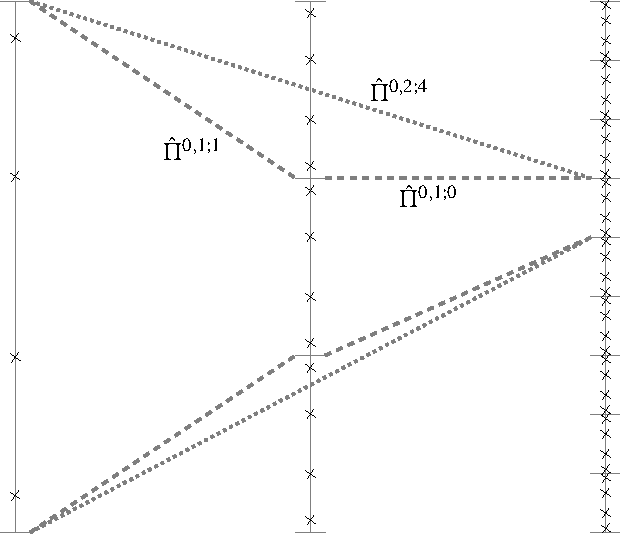
\includegraphics{amr_prolongation.pdf}
\caption[AMR prolongation]{Prolongation of coefficients from level $0$
down to level $2$. See
text for details on the prolongation operators. \textbf{TODO: Change to
top-down.}}
\label{fig:amr:prolongation}
\end{figure}
To this end, let us express the indices
$i^{0,l}=0,1,\ldots,3^l-1$
in terms of a tertiary basis:
\begin{align}
\label{eq:ader_impl:amr:subinterval_index}
i^{0,l} = \sum_{\beta=1}^{l}\,3^{l-\beta}\,j_\beta,\qquad j_\beta \in \{ 0,
1, 2 \}.
\end{align}

The support points and the corresponding
Lagrange basis functions
on the sub intervals can now be constructed in a recursive fashion
by downscaling and shifting the parent intervals:
\begin{align}
\hat{x}^{l;i^{0,l}}_k &= \frac{1}{3^l} (\hat{x}_k+i^{0,l})
= \frac{1}{3}\,(\hat{x}^{(l-1);i^{0,l-1}}_k+j_{l}), \\
\hat{\varphi}^{l;i^{0,l}}_k (\hat{x}) &=
\left(\prod_{\begin{smallmatrix}0\le n\le N\\ n\neq k\end{smallmatrix}}
\frac{\hat{x}-\hat{x}^{l;i^{0,l}}_n}{x^{l;i^{0,l}}_k-\hat{x}^{l;i^{0,l}}_n}\right),
\qquad k = 0,\ldots,N,
\end{align}
where $j_{l-1}\in\{0,1,2\}$ denotes the sub
interval index with respect to the parent interval.

The  level $0$ coefficients are then projected onto the $i^{0,l}$-th
subinterval of level $l$ in a recursive way similar to the way the 
subintervals are constructed, i.e.:
\begin{align}
\label{eq:amr:subinterval_recursion}
\hat{\Pi}^{0,l;i^{0,l}}_{m_0\,m_{l}}
&=
\sum_{m_{1}=0,\,m_{2}=0,\,\ldots,m_{l-1}=0}^N
\hat{\Pi}^{0,1;j_1}_{m_{0}\,m_{1}}\,
\ldots\,
\hat{\Pi}^{(l-2),(l-1);j_{l-1}}_{m_{l-2}\,m_{l-1}}\,\hat{\Pi}^{(l-1),l;j_l}_{m_{l-1}\,m_l}
\\
&=
\sum_{m_{1}=0,\,m_{2}=0,\,\ldots,m_{l-1}=0}^N
\hat{\Pi}^{0,1;j_1}_{m_{0}\,m_{1}}\,
\hat{\Pi}^{0,1;j_2}_{m_{1}\,m_{2}}\,
\ldots\,
\hat{\Pi}^{0,1;j_{l-1}}_{m_{l-2}\,m_{l-1}}\,\hat{\Pi}^{0,1;j_l}_{m_{l-1}\,m_l},
\end{align}
where $m_{0},m_{l}=0,1,\ldots,N$.

%%%%%%%%%%%%%%%%%%%%%%%%%%%%%%%%%%%%%%%%%%%%%%%%%%%%%%%%%%%%%%%%%%%%%%%%%%%%%%%
\section{Subcell prolongation and restriction operators}
\label{sec:amr:subcell_operators}
%%%%%%%%%%%%%%%%%%%%%%%%%%%%%%%%%%%%%%%%%%%%%%%%%%%%%%%%%%%%%%%%%%%%%%%%%%%%%%%
Subcell prolongation and restriction operators are important for the
prolongation and restriction of volume data in the context of dynamic
adaptive mesh refinement.

The prolongation operator can be simply constructed as tensor product of the
subinterval prolongation operators.

To this end, let us split the reference cell $\refCell=[0,1]^{d}$ into
$3^{l\,d}$, $l>0$, sub intervals
\begin{align}
\refCell^{l;i_l} = \frac{1}{3^{l}}[i_{l,1},\,i_{l,1}+1] \times
\frac{1}{3^{l}}[i_{l,2},i_{l,2}+1] \times \ldots \times
\frac{1}{3^{l}}[i_{l,{d}},\,i_{l,{d}}+1],
\end{align}
and let us further introduce a linear index
\begin{align}
\label{eq:ader_impl:amr:subface_index}
i^{0,l} = \sum_{\xi=1}^{d} I_{l,\xi}\,i_{l,\xi},
\end{align}
where the $I_{l,\xi}\in\{0,3^l\}$, $\xi \in \{1,2,\ldots,d\}$ denote some
strides that ensure the uniqueness of the index.

We can project coefficients associated with functions that
are constructed as $d$-dimensional tensor product
of the univariate basis functions onto the subcells
$\refCell^{l;i^{0,l}}$ by using a tensor product of the subinterval projectors
$\hat{\Pi}^{0,l;i^{0;l}_\xi}$, $\xi\in\{0,1,\ldots,d-1\}$
defined in the previous section:
\begin{align}
u^{l;i^{0,l}}_n
&=
\sum_{k'=0}^{(N+1)^{d}-1} u_{n'}\,
\frac{
\left\langle
\hat{\phi}_{n'},
\hat{\phi}^{l;i^{0,l}}
_{n}
\right\rangle
_{L^2(\refCell^{l;i^{0,l}})}
}
{
\left\langle
\hat{\phi}^{l;i^{0,l}}_{n}
\hat{\phi}^{l;i^{0,l}}_{n}
\right\rangle
_{L^2(\refCell^{l;i^{0,l}})}
}
\notag
\\
&=
\sum_{k'=0}^{(N+1)^{d}-1} u_{n'}\,
\prod_{\xi=1}^{d}
\frac{
\left\langle
\hat{\varphi}_{n'_\xi},
\hat{\varphi}^{l;i^{0,l}}_{n_\xi}
\right\rangle
_{L^2(\refCell^{l;i^{0,l}})}
}
{
\left\langle
\hat{\varphi}^{l;i^{0,l}}_{n_\xi}
\hat{\varphi}^{l;i^{0,l}}_{n_\xi}
\right\rangle
_{L^2(\refCell^{l;i^{0,l}})}
}
\notag
\\
&= \sum_{k'=0}^{(N+1)^{d}-1} u_{n'}\,\prod_{\xi=1}^{d}
\hat{\Pi}^{0,l;i^{0,l}_\xi}_{n'_\xi,n_\xi},\qquad n =
0,1,\ldots,(N+1)^{d}-1,
\end{align}
where the values $u_{n'}$, $n=0,\ldots,(N+1)^d$, denote coefficients
located at $d$-dimensional quadrature nodes on the reference element.  

\subsection{Restriction}
In the context of matrixfree nodal DG, the degrees of freedom of 
volume data $u_n$, $n=0,1,\ldots,(N+1)^d-1$, are located at the quadrature
nodes of a $d$-dimensional Gauss-Legendre quadrature.

We obtain from the $L^2$ projection of the 
subcell degrees of freedoms:
\begin{align}
u_n
&=
\sum_{i^{0,l}=0}^{3^{l\,d}-1}
\sum_{n'=0}^{(N+1)^{d}-1}
\prod_{\xi=1}^{d}\,
\frac{
\left\langle
\hat{\varphi}_{n_{\xi}},
\hat{\varphi}_{n'_{\xi}}^{l;i^{0;l}_\xi}
\right\rangle
_{L^2(\refCell^{0,l;i^{0;l}})}
}
{
\left\langle
\hat{\varphi}_{n_{\xi}},
\hat{\varphi}_{n_{\xi}}
\right\rangle
_{L^2(\refCell)}
}
\,u^{l;i^{0,l}}_{n'}
\\
&=
\sum_{i^{0,l}=0}^{3^{l\,d}-1}
\sum_{n'=0}^{(N+1)^{d}-1}
\prod_{\xi=1}^{d}\,
\frac{
\left\langle
\hat{\varphi}_{n_\xi},
\hat{\varphi}_{n'_\xi}^{l;i^{0;l}_\xi}
\right\rangle
_{L^2(\refCell^{0,l;i^{0;l}})}
}
{
\left\langle
\hat{\varphi}_{n_\xi},
\hat{\varphi}_{n_\xi}
\right\rangle
_{L^2(\refCell)}
}
\,
u^{l;i^{0,l}}_{n'}
\\
&=
\sum_{i^{0,l}=0}^{3^{l\,d}-1}
\sum_{n'=0}^{(N+1)^{d}-1}
\prod_{\xi=1}^{d}\,
\frac{
\frac{1}{3^{l}}\,
w_{n'_\xi}\,
\hat{\varphi}_{n_\xi}
\left(
\frac{1}{3^{l}} (\hat{x}_{n',\xi}+i_\xi^{0,l})
\right)
}
{
w_{n_\xi}
}
\,
u^{l;i^{0,l}}_{n'}
\\
&=
\sum_{i^{0,l}=0}^{3^{l\,d}-1}
\sum_{n'=0}^{(N+1)^{d}-1}
\frac{1}{3^{l\,d}}\,
\left(
\prod_{\xi=1}^{d}\,
\frac{w_{n'_\xi}}{w_{n_\xi}}\,
\hat{\Pi}^{0,l;i^{0,l}_\xi}_{n_\xi n'_\xi}
\right)
u^{l;i^{0,l}}_{n'}.
\end{align}

%%%%%%%%%%%%%%%%%%%%%%%%%%%%%%%%%%%%%%%%%%%%%%%%%%%%%%%%%%%%%%%%%%%%%%%%%%%%%%%
\section{Subface prolongation and restriction operators}
\label{sec:amr:subface_operators}
%%%%%%%%%%%%%%%%%%%%%%%%%%%%%%%%%%%%%%%%%%%%%%%%%%%%%%%%%%%%%%%%%%%%%%%%%%%%%%%
Subface projectors are important for performing the numerical flux
computation
on the interface between two mesh cells:
They are used to perform the prolongation and restriction
operation that is required if the two cells that share
the interface do not belong to the same refinement level.

Let us split the reference cell face $\hat{C}=[0,1]^{d-1}$ into $3^{l\,(d-1)}$
sub intervals
\begin{align}
\hat{C}^{l;i_l} = \frac{1}{3^l}[i_{l,1},\,i_{l,1}+1] \times
\frac{1}{3^l}[i_{l,2},i_{l,2}+1] \times \ldots \times
\frac{1}{3^l}[i_{l,{d-1}},\,i_{l,{d-1}}+1],
\end{align}
where the subinterval indices $i_{l,\zeta}=0,1,\ldots,3^l$, $\zeta\in\{0,1,d-1\}$
are defined by \eqref{eq:ader_impl:amr:subinterval_index}
,
and where we have introduced an unique index
\begin{align}
\label{eq:ader_impl:amr:subface_index}
i^{0,l} = \sum_{\zeta=1}^{d-1} I_{l,\zeta}\,i_{l,\zeta},
\end{align}
where the $I_{l,\zeta}\in\{0,3^l\}$, $\zeta \in \{1,2,\ldots,d-1\}$ denote some
strides that ensure the uniqueness of the index.

We can again project coefficients associated with functions that
are constructed as $(d-1)$-dimensional tensor product
of the univariate basis functions onto the subfaces
$C^{l;i^{0,l}}$ by using a tensor product of the subinterval projectors
$\hat{\Pi}^{0,l;i^{0;l}_\zeta}$, $\zeta\in\{0,1,\ldots,d-1\}$:
\begin{align}
g^{l;i^{0,l}}_k = \sum_{k'=0}^{(N+1)^{d-1}-1} g_{k'}\,\prod_{\zeta=1}^{d-1}
\hat{\Pi}^{0,l;i^{0,l}_\zeta}_{k'_\zeta,k_\zeta},\qquad k = 0,1,\ldots,(N+1)^{d-1}-1,
\end{align}
where the values $g_{k'}$, $k=0,\ldots,(N+1)^{d-1}-1$, denote coefficients
located at $(d-1)$-dimensional quadrature nodes located at the reference cell. 

\subsection{Restriction}
In the context of matrixfree nodal DG, the boundary extrapolated
values $g_k$, $k=0,1,\ldots,(N+1)^{d-1}-1$ are located at the quadrature
nodes of a ${d-1}$-dimensional Gauss-Legendre quadrature.

Since we can split the original integral over $\hat{C}=[0,1]^{d-1}$
into $3^{l\,(d-1)}$ integrals over each subface, the inverse operation
to the prolongation operation is to sum the integrals
over the subfaces.
The projection can thus be expressed as $L^2$-projection:
\begin{align} 
g_k
&\overset{\textup{(I)}}{=}
\sum_{i^{0,l}=0}^{3^{l\,(d-1)}-1}
\sum_{k'=0}^{(N+1)^{d-1}-1}
\prod_{\zeta=1}^{d-1}\,
\frac{
\left\langle
\hat{\varphi}_{k_\zeta},
\hat{\varphi}_{k'_\zeta}^{l;i^{0;l}_\zeta}
\right\rangle
_{L^2(\hat{C}^{0,l;i^{0;l}})}
}
{
\left\langle
\hat{\varphi}_{k_\zeta},
\hat{\varphi}_{k_\zeta}
\right\rangle
_{L^2(\hat{C})}
}
g^{l;i^{0,l}}_{k'}
\\
&=
\sum_{i^{0,l}=0}^{3^{l\,(d-1)}-1}
\sum_{k'=0}^{(N+1)^{d-1}-1}
\prod_{\zeta=1}^{d-1}\,
\frac{
\frac{1}{3^{l}}\,
w_{k'_\zeta}\,
\hat{\varphi}_{k_\zeta}
\left(
\frac{1}{3^{l}} (\hat{x}_{k',\zeta}+i_\zeta^{0,l})
\right)
}
{
w_{k_\zeta}
}
g^{l;i^{0,l}}_{k'}
\\
&=
\sum_{i^{0,l}=0}^{3^{l\,(d-1)}-1}
\sum_{k'=0}^{(N+1)^{d-1}-1}
\frac{1}{3^{l\,(d-1)}}\,
\left(
\prod_{\zeta=1}^{d-1}\,
\frac{w_{k'_\zeta}}{w_{k_\zeta}}\,
\hat{\Pi}^{0,l;i^{0,l}_\zeta}_{k_\zeta k'_\zeta}
\right)
g^{l;i^{0,l}}_{k'}.
\end{align}
\subsection{Determining the subface index from a subcell index}
For a given face $(\xi,f)$ of a cell on level $l-1$ and a single-level subcell
index $(c_1,c_2,\ldots,c_{d})$, $c_{\xi}\in\{0,1,2\}$,
$\xi\in\{0,1,\ldots,d\}$ we can reconstruct the single-level subface indices
$j_{l,\zeta}$, $\zeta\in\{0,1,\ldots,d-1\}$ according to Table
\ref{tab:ader_impl:amr:map_face_index_to_subcell_indices}.

With respect to the topmost face at level $l=0$
that contains the subface at level $l$, we
can then construct a projector for the respective subface
by recursively (bottom-up) determining the subface indices of all
intermediate levels and then computing an index (top-down) according to
\eqref{eq:ader_impl:amr:subface_index} and
\eqref{eq:ader_impl:amr:subinterval_index}
\begin{table}
\centering
\footnotesize
\renewcommand*{\arraystretch}{1.5}
\begin{tabular}{c|rrrrrrr}
$(\xi,f)$ & $(0,0)$ & $(0,1)$ & $(1,0)$ & $(1,1)$ & $(2,0)$ & $(2,1)$ & $\cdots$
\\
\hline
$c_{1}$ & 0 & 2 & $\in\{0,1,2\}$ & $\in\{0,1,2\}$ & $\in\{0,1,2\}$ &
$\in\{0,1,2\}$ & $\cdots$
\\
$c_{2}$ & $\in\{0,1,2\}$ & $\in\{0,1,2\}$ & 0 & 2 & $\in\{0,1,2\}$ & $\in\{0,1,2\}$
& $\cdots$
\\
$c_{3}$ & $\in\{0,1,2\}$ & $\in\{0,1,2\}$ & $\in\{0,1,2\}$ & $\in\{0,1,2\}$ & 0 & 2
& $\cdots$
\\
$\vdots$ & $\vdots\ddots$ & $\ddots$ & $\ddots$ & $\ddots$ & $\ddots$ & $\ddots$
& $\ddots$
\end{tabular}
\caption{Indices $(c_1,c_2,\ldots,c_d)$ of subcells that are adjacent
to the parent cell face with index $(\xi,f)$. The difference
in levels of the subcells and the parent cell is 1.}
\label{tab:ader_impl:amr:map_face_index_to_subcell_indices}
\end{table}

\section{Remarks on the ExaHyPE implementation}
\begin{enumerate}
  \item \textbf{Three additional DG operators:} Need to store the three
  order-dependent projectors $\hat{\Pi}^{0,1;j}\in\mathbb{R}^{(N+1)\times(N+1)}$
with
\begin{align}
\hat{\Pi}^{0,1;j}_{mn}
&=
\varphi_m \left( \frac{1}{3} (\hat{x}_n+j)\right),
\quad m,n=0,1,\ldots,N,
\end{align}
where $j\in\{0,1,2\}$.
Remark: This can be done with a lookup table similar to the one for \texttt{Kxi}.
\item \textbf{Face data restriction} is performed over multiple levels. 
We want to do that in a recursive fashion; cf.
\eqref{eq:amr:subinterval_recursion}.
We thus
need to implement a face data restriction operator such that:
\begin{align}
g_k &=
\sum_{i^{0,l}=0}^{3^{l\,(d-1)}-1}
\left(
\sum_{k'=0}^{(N+1)^{d-1}-1}
\frac{1}{3^{l\,(d-1)}}\,
\prod_{\zeta=1}^{d-1}\,
\frac{w_{k'_\zeta}}{w_{k_\zeta}}\,
\hat{\Pi}^{0,l;i^{0,l}_\zeta}_{k_\zeta k'_\zeta}
\,
g^{l;i^{0,l}}_{k'}
\right)
,
\end{align}
where $k=1,\ldots,(N+1)^{d-1}-1$.
The values $g_{k}$, $k=0,\ldots,(N+1)^{d-1}-1$, denote coefficients
associated with $(d-1)$-dimensional quadrature nodes on the face
of the coarse grid cell.

The values $g^{l;i^{0,1}}_{k'}$, $k'=0,\ldots,(N+1)^{d-1}-1$, denote
coefficients associated with $(d-1)$-dimensional quadrature nodes on the boundary
of the fine grid cell. 

Note that in the above notation level 0 refers
denotes the coarse grid level $l_\textup{coarse}$ and level $l$ refers to
the fine grid level $l_\textup{fine}$.

Since we loop over all subcells/subfaces in
the spacetree code, only the part in
the brackets has to be implemented on the solver side.

The spacetree code supplies the restriction
routine with the subinterval indices
$i^{0,l}_\zeta\in\{0,1,\ldots,3^l-1\}$, $\zeta\in\{1,2,\ldots,d-1\}$. 
These indices are encoded 
in terms of a tertiary basis:
\begin{align}
\label{eq:ader_impl:amr:subinterval_index}
i^{0,l}_\zeta = \sum_{\beta=1}^{l}\,3^{l-\beta}\,j_{\beta,\zeta},\qquad
j_{\beta,\zeta} \in \{ 0, 1, 2 \}.
\end{align}
The ``basis vector'' of the first projection level ($\beta=1$) is $3^{l-1}$,
the ``basis vector'' of the second projection level is
$3^{l-2}$, and so on.
This can be used to
reconstruct the sequence of subintervals
$\{j_1,j_2,j_3,j_4,\ldots,j_l\}$

A straightforward decoding of the subinterval indices
$i^{0,l}_\zeta$
would thus work like this:
\\
0. Allocate extra memory to store intermediate results.
We need to perform a chain of $l_\textup{fine}-l_\textup{coarse}-1$ MatVecs.
\\
1. Initialise fine grid values or temporay vector as coarse grid values.
\\
2. The solver code loops from 1 to up to the level
difference $l_\textup{fine}-l_\textup{coarse}$.
In each iteration, it has then to determine the 
indices $j_{\beta,}$ (how many $3^{l-\beta}$?), restrict the fine grid data by
one level and write the result to
the temporary vector or the fine grid values
in an alternating manner.
\item \textbf{Face data prolongation} is performed over multiple levels.
We want to do that in a recursive fashion; cf.
\eqref{eq:amr:subinterval_recursion}.
We thus need to implement a face data prolongation operator such that:
\begin{align}
g^{l;i^{0,l}}_k = \sum_{k'=0}^{(N+1)^{d-1}-1} g_{k'}\,\prod_{\zeta=1}^{d-1}
\hat{\Pi}^{0,l;i^{0,l}_\zeta}_{k'_\zeta,k_\zeta},\qquad k =
0,1,\ldots,(N+1)^{d-1}-1.
\end{align}
See above for a definition of the symbols.

\item \textbf{Volume data restriction} is performed over multiple levels. 
We want to do that in a recursive fashion; cf.
\eqref{eq:amr:subinterval_recursion}.
We thus need to implement a volume  data restriction operator such that:
\begin{align}
u_n &=
\sum_{i^{0,l}=0}^{3^{l\,d}-1}
\left(
\sum_{n'=0}^{(N+1)^{d}-1}
\frac{1}{3^{l\,d}}\,
\prod_{\zeta=1}^{d}\,
\frac{w_{n'_\zeta}}{w_{n_\zeta}}\,
\hat{\Pi}^{0,l;i^{0,l}_\zeta}_{n_\zeta n'_\zeta}
\,
u^{l;i^{0,l}}_{n'}
\right)
,
\end{align}
where $n=1,\ldots,(N+1)^{d}-1$.
The values $u_{n}$, $k=0,\ldots,(N+1)^{d}-1$, denote coefficients
associated with $d$-dimensional quadrature nodes belonging to the coarse grid
cell.

The values $u^{l;i^{0,1}}_{n'}$, $n'=0,\ldots,(N+1)^{d}-1$, denote
coefficients associated with $d$-dimensional quadrature nodes belonging 
to the fine grid cell. 

Note that in the above notation level 0 refers
denotes the coarse grid level $l_\textup{coarse}$ and level $l$ refers to
the fine grid level $l_\textup{fine}$.

Since we loop over all subcells/subfaces in
the spacetree code, only the part in
the brackets has to be implemented on the solver side.

The spacetree code supplies the restriction
routine with the subcell indices
$i^{0,l}_\zeta\in\{0,1,\ldots,3^l-1\}$, $\zeta\in\{1,2,\ldots,d\}$. 
These indices are encoded 
in terms of a tertiary basis:
\begin{align}
\label{eq:ader_impl:amr:subinterval_index}
i^{0,l}_\zeta = \sum_{\beta=1}^{l}\,3^{l-\beta}\,j_{\beta,\zeta},\qquad
j_{\beta,\zeta} \in \{ 0, 1, 2 \}.
\end{align}
The ``basis vector'' of the first projection level ($\beta=1$) is $3^{l-1}$,
the ``basis vector'' of the second projection level is
$3^{l-2}$, and so on.
This can be used to
reconstruct the sequence of subintervals
$\{j_1,j_2,j_3,j_4,\ldots,j_l\}$.
\item \textbf{Volume data prolongation} is performed over multiple levels.
We want to do that in a recursive fashion; cf.
\eqref{eq:amr:subinterval_recursion}.
We thus need to implement a volume data prolongation operator
such that:
\begin{align}
u^{l;i^{0,l}}_n = \sum_{n'=0}^{(N+1)^{d}-1} u_{n'}\,\prod_{\zeta=1}^{d}
\hat{\Pi}^{0,l;i^{0,l}_\zeta}_{n'_\zeta,n_\zeta},\qquad n =
0,1,\ldots,(N+1)^{d}-1.
\end{align}
See above for a definition of the symbols.
\end{enumerate}

\end{document}
